% \iffalse meta-comment
%
% Copyright (C) 2022 by Sebastien Laclau
% -----------------------------------
%
% This file may be distributed and/or modified under the
% conditions of the LaTeX Project Public License, either version 1.3c
% of this license or (at your option) any later version.
% The latest version of this license is in:
%
% http://www.latex-project.org/lppl.txt
%
% and version 1.3c or later is part of all distributions of LaTeX
% version 2008 or later.
%
% \fi
%
% \iffalse

% \section{Identification}
%
%    Announce the file name and its version:
%
%    \begin{macrocode}
%<default&all>\ProvidesFile{examx-default.clo}
%<OCRALevel&all>\ProvidesFile{examx-OCRALevel.clo}
%<OCRALevel&answerbook>\ProvidesFile{examx-OCRALevelanswerbook.clo}
%<OCRALevel&formulaesheet>\ProvidesFile{examx-OCRALevelformulae.clo}
%<advanced&answerbook>\ProvidesFile{examx-advancedanswerbook.clo}
%<veryadvanced&answerbook>\ProvidesFile{examx-veryadvancedanswerbook.clo}
%<WellyOCR&covers>\ProvidesFile{examx-WellyOCRcovers.clo}
%<*driver>
\ProvidesFile{examx-styles.dtx}
%</driver>
	[2022/05/09 v1.1.3
%<!driver> standard latex class option file]
%<*driver>
]
\documentclass{ltxdoc}
%    \end{macrocode}
%    Some things do not need indexing.
%    \begin{macrocode}
\DoNotIndex{\AtEndOfClass, \AtEndEnvironment}
\DoNotIndex{\def, \gdef, \xdef, \let, \relax, \newif, \newcommand,
\renewcommand, \NewDocumentCommand, \RenewDocumentCommand}
\DoNotIndex{\,, \\, \vspace, \par, \baselineskip}
\DoNotIndex{\hline}
\DoNotIndex{\normalsize, \large, \Large, \LARGE, \huge}
\DoNotIndex{\bfseries, \textsc, \textcolor, \rm, \bf}
\DoNotIndex{\csname{else}, \cs{fi}}
\DoNotIndex{\csname{loop}, \csname{repeat}, \foreach, \breakforeach,
\m, \n, \x, \s}
\DoNotIndex{\begin, \end}
\DoNotIndex{\arabic, \alph, \Alph}
\DoNotIndex{\newcounter, \setcounter, \pgfmathsetcounter, \addtocounter}
\DoNotIndex{\lpos, \mpos, \rpos, \blankrow, \pageendrule,
\pagestartrule}
\DoNotIndex{\csname, \endcsname}
%    \end{macrocode}
%    We do want an index, using line numbers, and a change log.
%    \begin{macrocode}
\EnableCrossrefs
\CodelineIndex
\RecordChanges
%    \end{macrocode}
%    The following code retrieves the date and version information from
%the file.
%    \begin{macrocode}
\GetFileInfo{examx-styles.dtx}
%    \end{macrocode}
%    Here are some commonly used abbreviations:
%    \begin{macrocode}
\newcommand*{\Lopt}[1]{\textsf {#1}}
\newcommand*{\file}[1]{\texttt {#1}}
\newcommand*{\Lcount}[1]{\textsl {\small#1}}
\newcommand*{\pstyle}[1]{\textsl {#1}}
%    \end{macrocode}
%    We also want the full details.
%    \begin{macrocode}
\begin{document}
	\DocInput{examx-styles.dtx}
	\PrintIndex
	\PrintChanges
\end{document}
%</driver>
%    \end{macrocode}
%
% \fi
%
% \CheckSum{0}
%
% \changes{v1.0}{2022/01/31}{Initial version}
% \changes{v1.1.1}{2022/02/03}{Start of semver}
% \changes{v1.1.2}{2022/03/10}{Implemented \Lopt{fourside}}
%
%
%
% \title{Styles for the \textsf{examx} class\thanks{This document
	% corresponds to \file{examx-styles.dtx}~\fileversion,
	% dated \filedate.}}
% \author{Sebastien Laclau \\ \texttt{slaclau@wellingtoncollege.org.uk} \\ \texttt{seb.laclau@gmail.com}}
%
% \maketitle
%
% \tableofcontents
%
% \StopEventually{}
% \section{The {\sc docstrip} modules}
%
% The following modules are used in the implementation to direct
% {\sc docstrip} in generating the external files. The first set refer
%to styles, complete or incomplete. The next set are secondary guards
%used to separate between parts of a style and the whole style.
%Finally,
%there is the driver guard:
% \begin{center}
    % \begin{tabular}{p{0.3\textwidth}p{0.6\textwidth}}
        %   default             & produce the style used by default \\
        %   OCRALevel           & imitates the style of an OCR A Level
        %paper \\
        %   WellyOCR            & incomplete style used for covers only
        %\\
        %   advanced            & incomplete style used for answerbook
        %only \\
        %   veryadvanced        & incomplete style used for answerbook
        %only \\
        % \hline
        %   all                 & included in the complete style \\
        %   covers              & included in the cover style \\
        %   answerbook          & included in the answer book style \\
        %   formulaesheet       & included in the formulae sheet style
        %\\
        %   answerbookbackcover & used to include the default answer
        %book back covers in other styles \\
        % \hline
        %   driver        & produce a documentation driver file
        % \end{tabular}
    % \end{center}
%
%\section{Complete styles}
%\subsection{Default style}
%    \begin{macrocode}
%<*default>
\solndots

\renewcommand{\questionpaperend}{
    \footer{}{}{}
    \begin{center}
        \ifprintanswers {\bfseries END OF MARKSCHEME} \else {\bfseries
            END OF QUESTION PAPER} \fi
        \oddeven{\newpage {\bfseries This page is intentionally
                blank}}{}
        \ifexamx@fourside
        \ifnum\the\numexpr(\thepage/4)*4-\thepage\relax=2
        \newpage {\bfseries This page is intentionally blank}
        \newpage {\bfseries This page is intentionally blank}
        \fi
        \fi
    \end{center}
}
%    \end{macrocode}
%\subsubsection{Answer book}
%    \begin{macrocode}
%<*answerbookbackcover|answerbook|all>
\renewcommand{\answerbookbackcover}{
    \begin{center}
        \large\bfseries ADDITIONAL ANSWER SPACE
    \end{center}
    If additional space is required, you should use the following lined
    page(s). The question number(s) must be clearly shown in the
    margin(s).
    \fillwithdottedlines{\stretch{1}}
    \ifexamx@fourside
        \ifnum\the\numexpr(\thepage/4)*4-\thepage\relax=2
            \newpage
            \fillwithdottedlines{\stretch{1}}
            \newpage
            \fillwithdottedlines{\stretch{1}}
        \fi
    \fi
}
\renewcommand{\doubleanswerbookbackcover}{
    \begin{center}
        \large\bfseries ADDITIONAL ANSWER SPACE
    \end{center}
    If additional space is required, you should use the following lined
    page(s). The question number(s) must be clearly shown in the
    margin(s).
    \fillwithdottedlines{\stretch{1}}
    \newpage
    \fillwithdottedlines{\stretch{1}}
    \ifexamx@fourside
        \ifnum\the\numexpr(\thepage/4)*4-\thepage=2
            \newpage
            \fillwithdottedlines{\stretch{1}}
            \newpage
            \fillwithdottedlines{\stretch{1}}
        \fi
    \fi
}
%</answerbookbackcover|answerbook|all>
%</default>
%    \end{macrocode}
%\subsection{OCRALevel style}
%\subsubsection{Initial code}
%    The initial code configures various features of the examx
%class.
%    \begin{macrocode}
%<*OCRALevel>
%<*all>
\@alwaysdroppointsatright
\soln

\sisetup{inter-unit-product = \,}

\setmainfont[Ligatures=TeX]{TeX Gyre Termes}
\setmathfont[math-style=ISO,bold-style=ISO]{TeX Gyre Termes Math}
\setsansfont{Arial}

\titleformat{\section}{\bfseries\centering}{Section \Alph{section}:
}{0pt}{}[\@storequestiondata{\arabic{section}}{1}{-1}{0}
\label{sec:\Alph{section}}
]

\newgeometry{left=0.86 in,right=1.14 in,top=1 in,bottom=1 in}
\savegeometry{main}
\newgeometry{left=0.68 in,right=0.68 in,top=1 in,bottom=1 in}
\savegeometry{answerbook}
\loadgeometry{main}


\footer{}{}{\bfseries\oddeven{Turn over}{}}
\header{}{\bfseries \thepage}{}


\renewcommand{\questionstart}{
    \ifprintanswers \else
    \begin{center}
        Answer {\bfseries all} the questions.
    \end{center}
    \fi
}
\renewcommand{\questionshook}{\setlength{\itemsep}{1in}}
\renewcommand{\partshook}{\setlength{\topsep}{\baselineskip}
\setlength{\itemsep}{\baselineskip}}
\renewcommand{\solnorhook}{
    \renewcommand{\partshook}{\setlength{\itemsep}{\baselineskip}}
}

\renewcommand{\questionlabel}{\bfseries\thequestion.}
\renewcommand{\partlabel}{\bfseries(\thepartno)}
\renewcommand{\subpartlabel}{\bfseries(\thesubpart)}
\renewcommand{\subsubpartlabel}{\bfseries(\thesubsubpart)}

\pointname{}
\pointformat{\bfseries[\thepoints]}

\renewcommand{\vec}[1]{{\bf#1}}
\newcommand{\detailedreasoning}{\textbf{In this question you must show detailed reasoning.} \par }
%</all>
\DeclareMathOperator{\varexpec}{E}
\DeclareMathOperator{\varprob}{P}
\RequirePackage{lscape}
\RequirePackage{afterpage}
\RequirePackage{multirow}
\RequirePackage{enumitem}
\RequirePackage{xstring}
\RequirePackage{microtype}
%    \end{macrocode}
%
%\subsubsection{Covers}
%\begin{macro}{\examcover}
%    This code redefines the front cover of the question paper.
%    \begin{macrocode}
\usetikzlibrary{fit}
\renewcommand{\examcover}{
    \newgeometry{top=1.5cm, bottom=1cm, left=2.8cm, right=2.2cm}
    \thispagestyle{empty}
    \if\@logo\relax\else\includegraphics[height=2cm]{\@logo}\fi
    
    \vspace{2mm}
    
    {\sffamily
    
    {\LARGE \textbf{\@examdate}}
    
    \vspace{8pt}
    
    {\Large \textbf{\@examtitle}}
    
    \vspace{8pt}
    
    {\large \unless\if\@examcode\relax\textbf{\@examcode} $\quad$\fi\@examtopic}
    
    \vspace{8pt}
    
    {\normalsize \textbf{Time allowed: \@examtime}}
    
    \vspace{12pt}
    
    \begin{tikzpicture}
    \node[draw, text width=7.87cm, text depth=4.19cm, rounded corners] at (0,0) {
        {\footnotesize
            \textbf{You must have:}
            
            \ifanswerbook$\bullet$ Printed Answer Booklet \\ \fi
            \ifcalculatorrequired$\bullet$ a scientific or graphical calculator \\ \fi
            
            \ifcalculator
            \vspace*{.5cm}
            
            \textbf{You may use:}
            
            $\bullet$ a scientific or graphical calculator \\
            
            \fi
        }
    };
    \end{tikzpicture}
    \vspace{0.6cm}
    
    \small
        \textbf{INSTRUCTIONS}
        \begin{itemize}[nolistsep]
            \item Use black ink. You can use a HB pencil but only for graphs and diagrams.
            \item Write your answer to each question in the space provided in the \textbf{Printed Answer Booklet.} If you need extra space use the lined pages at the end of the Printed Answer Booklet. The question numbers must be clearly shown.
            \item Fill in the boxes on the front of the Printed Answer Booklet.
            \item Answer \textbf{all} the questions.
            \item Where appropriate, your answer should be supported with working. Marks might be given for using a correct method, even if your answer is wrong.
            \item Give non-exact numerical answers correct to 3 significant figures unless a different degree of accuracy is specified in the question
            \ifcalculator \item You are permitted to use a
            scientific or graphical calculator in this paper.
            \else \unless\ifcalculatorrequired \item You are not permitted to use a calculator in this paper. \fi \fi
            \item The acceleration due to gravity is denoted by $\grav\,\unit{\m\per\s\squared}$. Unless otherwise instructed, when a numerical value is needed, use $\grav=9.8$.
            \item Do \textbf{not} send this Question Paper for marking. Keep it in the centre or recycle it.
        \end{itemize}
        \vspace{4mm}
        \small
    
        \textbf{INFORMATION}
        \begin{itemize}[nolistsep]
            \item The total mark for this paper is  {\bfseries \thetotalpoints}.
            \item The marks for each question are shown in
            brackets {\bfseries [ ]}.
            \item This document consists of {\bfseries
                \pageref{lastpageofquestionpaper}} pages.
            \unless\if\@extrainfo\relax
            \item {\let \\ \item \@extrainfo}
            \fi
        \end{itemize}
        \vspace{4mm}
        \small
        
        \textbf{ADVICE}
        \begin{itemize}[nolistsep]
            \item Read each question carefully before you start an answer.
            \if\@extraadvice\relax\else
            \item {\let \\ \item \@extraadvice}
            \fi
        \end{itemize}
    \vfill
    \hfill{\footnotesize \textbf{Turn over}}}
    \newpage
    \loadgeometry{main}
    \ifprintanswers \else \ifexamx@formulae
    \formulaesheet \fi \fi
}
%    \end{macrocode}
%\end{macro}
%\begin{macro}{\answerbookcover}
%    This code redefines the front cover of the answer book.
%    \begin{macrocode}
\renewcommand{\answerbookcover}{
    \newgeometry{top=1.5cm, bottom=1cm, left=2.8cm, right=2.2cm}
    \thispagestyle{empty}
    \if\@logo\relax\else\includegraphics[height=2cm]{\@logo}\fi
    
    \vspace{2mm}
    
    {\sffamily
        
        {\LARGE \textbf{\@examdate}}
        
        \vspace{8pt}
        
        {\Large \textbf{\@examtitle}}
        
        \vspace{8pt}
        
        {\large \unless\if\@examcode\relax\textbf{\@examcode} $\quad$\fi\@examtopic}
        
        \vspace{8pt}
        
        {\large Printed Answer Book}
        
        \vspace{8pt}
        
        {\normalsize \textbf{Time allowed: \@examtime}}
        
        \vspace{12pt}
        
        \begin{tikzpicture}
        \node[draw, text width=7.87cm, text depth=3.18cm, rounded corners] at (0,0) {
            {\footnotesize
                \textbf{You must have:}
                
                \ifanswerbook$\bullet$ Printed Answer Booklet \\ \fi
                \ifcalculatorrequired$\bullet$ a scientific or graphical calculator \\ \fi
                
                \ifcalculator
                \vspace*{.5cm}
                
                \textbf{You may use:}
                
                $\bullet$ a scientific or graphical calculator \\
                
                \fi
            }
        };
        \end{tikzpicture}
        
        \setlength{\fboxsep}{0pt}
        \newcommand\abox{%
            \raisebox{-3mm}{\framebox[9.4mm]{\vline width 0mm height 9.4mm}}%
        }
    
    
        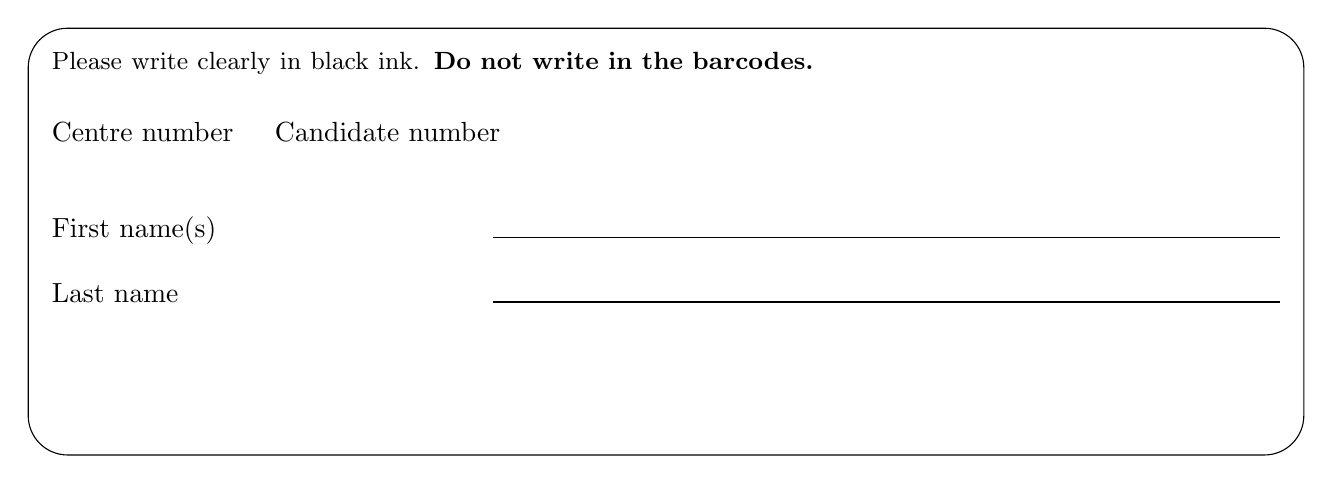
\begin{tikzpicture}
        \node[draw, text width=15.6cm, text depth=4.60cm, rounded corners=0.5cm, inner sep=0.3cm] at (0,0) {
            \normalsize {\small Please write clearly in black ink. \textbf{Do not write in the barcodes.}}
            
            \vspace{0.5cm}
            
            Centre number \abox\abox\abox\abox\abox \enspace\enspace\thinspace Candidate number \abox\abox\abox\abox
            
            \vspace{0.8cm}
            
            First name(s) \hspace{\stretch{1}} \rule{10cm}{0.15mm}
            
            \vspace{0.4cm}
            
            Last name \hspace{\stretch{1}} \rule{10cm}{0.15mm}
        };
        \end{tikzpicture}
        
        \small
        \textbf{INSTRUCTIONS}
        \begin{itemize}[nolistsep]
            \item Use black ink. You can use a HB pencil but only for graphs and diagrams.
            \item Write your answer to each question in the space provided in the \textbf{Printed Answer Booklet.} If you need extra space use the lined pages at the end of the Printed Answer Booklet. The question numbers must be clearly shown.
            \item Fill in the boxes on the front of the Printed Answer Booklet.
            \item Answer \textbf{all} the questions.
            \item Where appropriate, your answer should be supported with working. Marks might be given for using a correct method, even if your answer is wrong.
            \item Give non-exact numerical answers correct to 3 significant figures unless a different degree of accuracy is specified in the question
            \ifcalculator \item You are permitted to use a
            scientific or graphical calculator in this paper.
            \else \unless\ifcalculatorrequired \item You are not permitted to use a calculator in this paper. \fi \fi
            \item The acceleration due to gravity is denoted by $\grav\,\unit{\m\per\s\squared}$. Unless otherwise instructed, when a numerical value is needed, use $\grav=9.8$.
        \end{itemize}
        \vspace{4mm}
        \small
        
        \textbf{INFORMATION}
        \begin{itemize}[nolistsep]
            \item The total mark for this paper is  {\bfseries \thetotalpoints}.
            \item The marks for each question are shown in
            brackets {\bfseries [ ]}.
            \item This document consists of {\bfseries
                \pageref{lastpageofquestionpaper}} pages.
            \unless\if\@extrainfo\relax
            \item {\let \\ \item \@extrainfo}
            \fi
        \end{itemize}
        \vspace{4mm}
        \small
        
        \textbf{ADVICE}
        \begin{itemize}[nolistsep]
            \item Read each question carefully before you start an answer.
            \if\@extraadvice\relax\else
            \item {\let \\ \item \@extraadvice}
            \fi
        \end{itemize}
        \vfill
        \hfill{\footnotesize \textbf{Turn over}}}
    \newpage
    \loadgeometry{main}
}
%    \end{macrocode}
%\end{macro}
%\changes{v1.13}{2022/05/23}{Added cover for OCR A Level -- thanks to JCB}
%\subsubsection{Formulae sheet}
%\begin{macro}{\formulaesheet}
%    This code redefines the formulae sheet.
%    \begin{macrocode}
%<*formulaesheet|all>
\newgeometry{left=0.86 in,right=0.86 in,top=1 in,bottom=1 in}
\savegeometry{formulaesheet}
\loadgeometry{main}
\def\preheading{\vspace{0.15 in}}
\def\postheading{\vspace{0.08 in}}
\newcommand{\heading}[1]{\preheading {\bfseries #1} \par \postheading}
\newcommand{\topheading}[1]{{\large\bfseries #1} \par}
% Copyright (C) 2022 by Sebastien Laclau
% -----------------------------------
%
% This file may be distributed and/or modified under the
% conditions of the LaTeX Project Public License, either version 1.3c
% of this license or (at your option) any later version.
% The latest version of this license is in:
%
% http://www.latex-project.org/lppl.txt
%
% and version 1.3c or later is part of all distributions of LaTeX
% version 2008 or later.

\renewcommand{\formulaesheet}{
    \loadgeometry{formulaesheet}
    \def\preheading{\vspace{0.25 in}}
    \def\postheading{\vspace{0.08 in}}
    \begin{center}
        {\bfseries Formulae \par A Level Mathematics A (H240)}
    \end{center}
    \begin{flushleft}
        \heading{Arithmetic series}
        $S_n=\frac{1}{2}n(a+l)=\frac{1}{2}n\{2a+(n-1)d\}$ \par
        \heading{Geometric series}
        $S_n=\dfrac{a(1-r^n)}{1-r}$ \par
        $S_\infty=\dfrac{a}{1-r}$ for $\abs{r}<1$ \par
        \heading{Binomial series}
        $(a+b)^n=a^n+\prescript{n}{}{C_1}a^{n-1}b+\prescript{n}{}{C_2}
        a^{n-2}b^2+\ldots+\prescript{n}{}{C_r}a^{n-r}b^r+\ldots+b^n$
        \quad ($n\in\nats$), where
        $\prescript{n}{}{C_r}=\colvec{n\\r}=\dfrac{n!}{r!(n-r)!}$ \par
        $(1+x)^n=1+nx+\dfrac{n(n-1)}{2}x^2+\ldots+\dfrac{n(n-1)
            \dots(n-r+1)}{r!}x^r+\ldots$ \quad ($\abs{x}<1$) \par
        \heading{Differentiation}
        \begin{tabular}{|p{2.56 in}|p{2.56 in}|}
            \multicolumn{1}{l}{$f(x)$} & \multicolumn{1}{l}{$f'(x)$} \\
            \hline
            $\tan kx$ & $k\sec^2 kx$ \\ \hline
            $\sec x$ & $\sec x \tan x$ \\ \hline
            $\cot x$ & $-\csc^2 x$ \\ \hline
            $\csc x$ & $-\csc x \cot x$ \\ \hline
        \end{tabular}

        \vspace{.1 in}
        Quotient rule $y=\dfrac{u}{v}$,
        $\dydx=\dfrac{v\dudx-u\dvdx}{v^2}$ \par

        \heading{Differentiation from first principles}
        $f'(x)=\lim_{h\to0}\frac{f(x+h)-f(x)}{h}$ \par

        \heading{Integration}
        $\displaystyle\int\frac{f'(x)}{f(x)}\,\dx=\ln\abs{f(x)}+c$ \par
        $\displaystyle\int f'(x)(f(x))^n\,\dx=
        \dfrac{1}{n+1}(f(x))^{n+1}+c$ \par
        Integration by parts $\displaystyle\int u\dvdx\,\dx=
        uv-\int v\dudx\,\dx$ \par

        \heading{Small angle approximations}
        $\sin\theta\approx\theta$, $\cos\theta=1-\frac{1}{2}\theta^2$,
        $\tan\theta=\theta$ where $\theta$ is measured in radians
        \newpage
        \heading{Trigonometric identities}

        $\sin(A\pm B)=\sin A\cos B\pm \cos A\sin B$
        $\phantom{\dfrac{\tan A\pm\tan B}{1\mp\tan A\tan B}}$ \par
        $\cos(A\pm B)=\cos A\cos B\mp \sin A\sin B$
        $\phantom{\dfrac{\tan A\pm\tan B}{1\mp\tan A\tan B}}$ \par
        $\tan(A\pm B)=\dfrac{\tan A\pm\tan B}{1\mp\tan A\tan B}$ \quad
        $\left(A\pm B\neq (k+\frac{1}{2}\pi)\right)$ \par

        \heading{Numerical methods}
        Trapezium rule: $\int_a^b y\,\dx\approx
        h\{(y_0+y_n)+2(y_1+y_2+\ldots+y_{n-1})\}$, where
        $h=\dfrac{b-a}{n}$ \par
        The Newton-Raphson iteration for solving $f(x)=0$:
        $x_{n+1}=x_n-\dfrac{f(x_n)}{f'(x_n)}$ \par

        \heading{Probability}
        $\varprob(A\cup B)=\varprob(A)+\varprob(B)-\varprob(A\cap B)$
        \par
        $\varprob(A\cap B)
        =\varprob(A)\varprob(B|A)=\varprob(B)\varprob(A|B)$
        {\bfseries or}
        $\varprob(A|B)=\dfrac{\varprob(A\cap B)}{\varprob(B)}$ \par

        \heading{Standard deviation}
        $\sqrt{\dfrac{\sum(x-\bar{x})^2}{n}}=\sqrt{\dfrac{\sum
                x^2}{n}-\bar{x}^2}$ {\bfseries or} $\sqrt{\dfrac{\sum
                f(x-\bar{x})^2}{\sum f}}=\sqrt{\dfrac{\sum fx^2}{\sum
                f}-\bar{x}^2}$ \par

        \heading{The binomial distribution}
        If $X{\sim}B(n,p)$ then $\varprob(X=x)=
        \colvec{n \\ x}p^x(1-p)^{n-x}$,

        Mean of $X$ is $np$, Variance of $X$ is $np(1-p)$ \par

        \heading{Hypothesis test for the mean of a normal distribution}
        If $X{\sim}\mathrm{N}(\mu,\sigma^2)$ then
        $\bar{X}{\sim}\mathrm{N}\left(\mu,\dfrac{\sigma^2}{n}\right)$
        and $\dfrac{\bar{X}-\mu}{\sigma/\sqrt{n}}\sim \mathrm{N}(0,1)$
        \par

        \heading{Percentage points of the normal distribution}
        If $Z$ has a normal distribution with mean $0$ and variance $1$
        then, for each value of $p$, the table gives the value of $z$
        such that $\varprob(Z\leq z)=p$. \par
        \begin{center}
            \begin{tabular}{|c|c|c|c|c|c|c|c|c|c|}
                \hline
                $p$ & 0.75  & 0.90  & 0.95  & 0.975 & 0.99  & 0.995 &
                0.9975 & 0.999 & 0.9995 \\ \hline
                $z$ & 0.674 & 1.282 & 1.645 & 1.960 & 2.326 & 2.576 &
                2.807 & 3.090 & 3.291 \\ \hline
            \end{tabular}
        \end{center}

        \heading{Kinematics}
        {\setlength\tabcolsep{0 pt}
            \begin{tabular}{p{3 in} p{3 in}}

                Motion in a straight line & Motion in two dimensions \\
                $v=u+at$                  & $\vec{v}=\vec{u}+\vec{a}t$\\
                $s=ut+\frac{1}{2}at^2$    &
                $\vec{s}=\vec{u}+\frac{1}{2}\vec{a}t^2$ \\
                $s=\frac{1}{2}(u+v)t$     &
                $\vec{s}=\frac{1}{2}(\vec{u}+\vec{v})$ \\
                $v^2=u^2+2as$             & \\
                $s=vt-\frac{1}{2}at^2$    &
                $\vec{s}=\vec{v}-\frac{1}{2}\vec{a}t^2$
        \end{tabular}}
    \end{flushleft}
    \newpage
    \loadgeometry{main}
}
\newcommand{\mechformulae}{
    \begin{flushleft}
        \setlength{\parskip}{0.15 in}
        \penalty-20000
        \topheading{Mechanics}
        \nopagebreak
        \heading{Kinematics}
        \nopagebreak
        {\setlength\tabcolsep{0 pt}
            \begin{tabular}{p{3 in} p{3 in}}
                Motion in a straight line & Motion in two dimensions \\
                & \\
                $v=u+at$                  & $\vec{v}=\vec{u}+\vec{a}t$
                \\
                & \\
                $s=ut+\frac{1}{2}at^2$    &
                $\vec{s}=\vec{u}+\frac{1}{2}\vec{a}t^2$ \\
                & \\
                $s=\frac{1}{2}(u+v)t$     &
                $\vec{s}=\frac{1}{2}(\vec{u}+\vec{v})$ \\
                & \\
                $v^2=u^2+2as$             &
                $\vec{v}\cdot\vec{v}=
                \vec{u}\cdot\vec{u}+2\vec{a}\cdot\vec{s}$ \\
                & \\
                $s=vt-\frac{1}{2}at^2$    &
                $\vec{s}=\vec{v}-\frac{1}{2}\vec{a}t^2$
        \end{tabular}}

        \heading{Newton's experimental law}
        Between two smooth spheres $v_1-v_2=-e(u_1-u_2)$ \par
        Between a smooth sphere with a fixed plane surface $v=-eu$ \par

        \heading{Motion in a circle}
        Tangential velocity is $v=r\dot{\theta}$ \par
        Radial acceleration is $\frac{v^2}{r}$ or $r\dot{\theta}^2$
        towards the centre \par
        Tangential acceleration is $\dot{v}=r\ddot{\theta}$ \par

        \heading{Centres of mass}
        Triangular lamina: $\frac{3}{2}$ along median from vertex \par
        Solid hemisphere, radius $r$: $\frac{3}{8} r$ from centre \par
        Hemispherical shell, radius $r$:
        $\frac{1}{2} r$ from centre \par
        Circular arc, radius $r$, angle at centre $2\alpha$:
        $\frac{r\sin\alpha}{\alpha}$ from centre \par
        Sector of circle, radius $r$, angle at centre $2\alpha$:
        $\frac{2r\sin\alpha}{3\alpha}$ from centre \par
        Solid cone or pyramid of height $h$:
        $\frac{1}{4} h$ above the base on the line from centre of
        base to vertex \par
        Conical shell of height $h$:
        $\frac{1}{3} h$ above the base on the line from centre of
        base to vertex \par
    \end{flushleft}
    \clearpage
}

\newcommand{\pureformulae}{
    \begin{flushleft}
        \setlength{\parskip}{0.07 in}
        \topheading{Pure Mathematics}

        \heading{Arithmetic series}
        $S_n=\frac{1}{2}n(a+l)=\frac{1}{2}n\{2a+(n-1)d\}$ \par

        \heading{Geometric series}
        $S_n=\dfrac{a(1-r^n)}{1-r}$ \par
        $S_\infty=\dfrac{a}{1-r}$ for $\abs{r}<1$ \par

        \heading{Binomial series}
        $(a+b)^n=a^n+\prescript{n}{}{C_1}a^{n-1}b+
        \prescript{n}{}{C_2}a^{n-2}b^2+\ldots+
        \prescript{n}{}{C_r}a^{n-r}b^r+\ldots+b^n$
        \quad ($n\in\nats$), where
        $\prescript{n}{}{C_r}=
        \colvec{n\\r}=\dfrac{n!}{r!(n-r)!}$ \par
        $(1+x)^n=1+nx+\dfrac{n(n-1)}{2}x^2+\ldots+
        \dfrac{n(n-1)\dots(n-r+1)}{r!}x^r+\ldots$
        \quad ($\abs{x}<1$, $n\in\reals$) \par

        \heading{Series}
        $\displaystyle\sum_{r=1}^n r^2=\frac{1}{6}n(n+1)(2n+1)$,
        $\displaystyle\sum_{r=1}^n r^3=\frac{1}{4}n^2(n+1)^2$ \par

        \heading{Maclaurin series}
        $f(x)=f(0)+f'(0)x+\dfrac{f''(0)}{2!}x^2+\dots+
        \dfrac{f^{(r)}(0)}{r!}x^r+\dots$ \par
        $\e^x=\exp(x)=1+x+\dfrac{x^2}{2!}+\dots+\dfrac{x^r}{r!}+\dots$
        for all $x$ \par
        $\ln(1+x)=x=\dfrac{x^2}{2}+\dfrac{x^3}{3}-\dots+
        (-1)^{r+1} \dfrac{x^r}{r}+\dots$ ($-1<x<1$) \par
        $\sin x =x-\dfrac{x^2}{3!}+\dfrac{x^5}{5!}-\dots+
        (-1)^r \dfrac{x^{2r+1}}{(2r+1)!}+\dots$ for all $x$ \par
        $\cos x =1-\dfrac{x^2}{2!}+\dfrac{x^4}{4!}-\dots+
        (-1)^r\dfrac{x^{2r}}{2r!}+\dots$ for all $x$ \par
        $(1+x)^n=1+nx+\dfrac{n(n-1)}{2!}x^2+\dots+
        \dfrac{n(n-1)\dots(n-r+1)}{r!}x^r+\dots$ \quad
        ($\abs{x}<1$, $n\in\reals$) \par

        \heading{Matrix transformations}
        Reflection in the line $y=\pm x$:
        $\begin{pmatrix} 0 & \pm 1 \\ \pm 1 & 0 \end{pmatrix}$ \par
        Anticlockwise rotation through $\theta$ about $O$:
        $\begin{pmatrix} \cos\theta & -\sin\theta \\
            \sin\theta & \cos\theta \end{pmatrix}$ \par
        Rotations through $\theta$ about the coordinate axes. The
        direction of positive rotation is taken to be anticlockwise
        when looking towards the origin from the positive side of the
        axis of rotation.
        \begin{flalign*}
            R_x&=\begin{bmatrix} 1 & 0 & 0 \\
                0 & \cos\theta & -\sin\theta \\
                0 & \sin\theta & \cos\theta \end{bmatrix} &\\
            R_y&=\begin{bmatrix} \cos\theta & 0 & \sin\theta \\
                0 & 1 & 0 \\
                -\sin\theta & 0 & \cos\theta \end{bmatrix} &\\
            R_x&=\begin{bmatrix} \cos\theta & -\sin\theta & 0 \\
                \sin\theta & \cos\theta & 0 \\
                0 & 0 & 1 \end{bmatrix} &
        \end{flalign*}

        \heading{Differentiation}
        \newcolumntype{Y}{>{\centering\arraybackslash}X}
        \begin{tabularx}{\textwidth}{|Y|Y|}
            \multicolumn{1}{c}{$f(x)$} & \multicolumn{1}{c}{$f'(x)$} \\
            \hline
            $\tan kx$ & $k\sec^2 kx$ \\ \hline
            $\sec x$ & $\sec x \tan x$ \\ \hline
            $\cot x$ & $-\csc^2 x$ \\ \hline
            $\csc x$ & $-\csc x \cot x$ \\ \hline & \\[-0.2cm]
            $\arcsin x$ or $\sin^{-1}x$ & $\dfrac{1}{\sqrt{1-x^2}}$
            \\[0.5cm] \hline & \\[-0.2cm]
            $\arccos x$ or $\cos^{-1}x$ & $-\dfrac{1}{\sqrt{1-x^2}}$
            \\[0.5cm] \hline & \\[-0.2cm]
            $\arctan x$ or $\tan^{-1}x$ & $\dfrac{1}{1+x^2}$ \\[0.5cm]
            \hline
        \end{tabularx} \par


        \setlength{\parskip}{0.11 in}
        Quotient rule $y=\dfrac{u}{v}$,
        $\dydx=\dfrac{v\dudx-u\dvdx}{v^2}$\par

        \heading{Differentiation from first principles}
        $f'(x)=\lim_{h\to0}\dfrac{f(x+h)-f(x)}{h}$ \par

        \heading{Integration}
        $\displaystyle\int\frac{f'(x)}{f(x)}\,\dx=\ln\abs{f(x)}+c$ \par
        $\displaystyle\int
        f'(x)\left(f(x)\right)^n\,\dx=
        \dfrac{1}{n+1}\left(f(x)\right)^{n+1}+c$ \par
        Integration by parts $\displaystyle\int u\dvdx\dx=
        uv-\int v\dudx\dx$ \par
        The mean value of $f(x)$ on the interval $[a,b]$ is
        $\displaystyle\frac{1}{b-a}\int_a^b f(x)\dx$ \par
        Area of sector enclosed by polar curve is
        $\displaystyle\frac{1}{2}\int r^2 \dtheta$ \par

        \begin{tabular}{|c|c|}
            \multicolumn{1}{c}{$f(x)$} &
            \multicolumn{1}{c}{$\int f(x)\dx$} \\ \hline &
            \\[-0.2cm]
            $\dfrac{1}{\sqrt{a^2-x^2}}$ &
            $\sin^{-1}\left(\dfrac{x}{a}\right)$
            \quad$(\abs{x}<a)$ \\[0.5cm] \hline & \\[-0.2cm]
            $\dfrac{1}{a^2+x^2}$ &
            $\frac{1}{a}\tan^{-1}\left(\dfrac{x}{a}\right)$
            \\[0.5cm] \hline & \\[-0.2cm]
            $\dfrac{1}{\sqrt{a^2+x^2}}$ &
            $\sinh^{-1}\left(\dfrac{x}{a}\right)$ or
            $\ln(x+\sqrt{x^2+a^2})$ \\[0.5cm] \hline &
            \\[-0.2cm]
            $\dfrac{1}{\sqrt{x^2-a^2}}$ &
            $\cosh^{-1}\left(\dfrac{x}{a}\right)$ or
            $\ln(x+\sqrt{x^2-a^2})$ \\[0.5cm] \hline
        \end{tabular} \par

        \heading{Numerical methods}
        Trapezium rule: $\int_a^b y\,\dx\approx
        h\{(y_0+y_n)+2(y_1+y_2+\ldots+y_{n-1})\}$, where
        $h=\dfrac{b-a}{n}$ \par
        The Newton-Raphson iteration for solving $f(x)=0$:
        $x_{n+1}=x_n-\dfrac{f(x_n)}{f'(x_n)}$

        \heading{Complex numbers}
        Circles: $\abs{z-a}=k$ \par
        Half lines: $\arg{z-a}=\alpha$ \par
        Lines: $\abs{z-a}=\abs{z-b}$ \par
        De Moivre's theorem: $\{r(\cos\theta+i\sin\theta)\}^n=r^n(\cos
        n\theta+i\sin n\theta)$ \par
        Roots of unity: the roots of $z_n=1$ are given by
        $z=\exp\left(\frac{2\pi k}{n}i\right)$ for $k=0,1,2,\dots,n-1$
        \par

        \heading{Vectors and 3--D coordinate geometry}
        Cartesian equation of the line through the point $A$ with
        position vector $\vec{a}=a_1\vec{i}+a_2\vec{j}+a_3\vec{k}$ in
        direction $\vec{u}=u_1\vec{i}+u_2\vec{j}+u_3\vec{k}$ is
        $\dfrac{x-a_1}{u_1}=\dfrac{y-a_2}{u_2}=\dfrac{z-a_3}{u_3}(=\lambda)$
         \par
        Cartesian equation of a plane $n_1x+n_2y+n_3z+d=0$ \par
        Vector product
        $\vec{a}\times\vec{b}=\begin{pmatrix}a_1\\a_2\\a_3\end{pmatrix}\times\begin{pmatrix}b_1\\b_2\\b_3\end{pmatrix}=\begin{vmatrix}\vec{i}&a_1&b_1\\\vec{j}&a_2&b_2\\\vec{k}&a_3&b_3\end{vmatrix}=\begin{pmatrix}a_2b_3-a_3b_2\\a_3b_1-a_1b_3\\a_1b_2-a_2b_1\end{pmatrix}$
         \par
        The distance between skew lines is
        $D=\dfrac{\abs{(\vec{b}-\vec{a})\cdot\vec{n}}}{\abs{\vec{n}}}$,
        where $\vec{a}$ and $\vec{b}$ are position vectors of points on
        each line and $\vec{n}$ is a mutual perpendicular to both lines
        \par The distance between a point and a line is
        $D=\dfrac{\abs{ax_1+by_1-c}}{\sqrt{a^2+b^2}}$, where the
        coordinates of the point are (x1, y1) and the equation of the
        line is given by $ax+by+c$ \par
        The distance between a point and a plane is
        $D=\dfrac{\abs{\vec{b}\cdot\vec{n}-p}}{\abs{n}}$ where
        $\vec{b}$ is the position vector of the point and the equation
        of the plane is given by $\vec{r}\cdot\vec{n}=p$ \par

        \heading{Small angle approximations}
        $\sin\theta\approx\theta$, $\cos\theta=1-\frac{1}{2}\theta^2$,
        $\tan\theta=\theta$ where $\theta$ is measured in radians

        \heading{Trigonometric identities}
        $\sin(A\pm B)=\sin A\cos B\pm \cos A\sin B$
        $\phantom{\dfrac{\tan A\pm\tan B}{1\mp\tan A\tan B}}$ \par
        $\cos(A\pm B)=\cos A\cos B\mp \sin A\sin B$
        $\phantom{\dfrac{\tan A\pm\tan B}{1\mp\tan A\tan B}}$ \par
        $\tan(A\pm B)=\dfrac{\tan A\pm\tan B}{1\mp\tan A\tan B}$ \quad
        $\left(A\pm B\neq (k+\frac{1}{2}\pi)\right)$ \par

        \heading{Hyperbolic functions}
        $\cosh^2 x-\sinh^2 x=1$ \par
        $\sinh^{-1}x=\ln[x+\sqrt{(x^2+1)}]$ \par
        $\cosh^{-1}x=\ln[x+\sqrt{(x^2-1)}]$, $x\geq 1$ \par
        $\tanh^{-1}x=\dfrac{1}{2}\ln\left(\dfrac{1+x}{1-x}\right)$,
        $-1<x<1$ \par

        \heading{Simple harmonic motion}
        $x=A\cos\omega t+B\sin\omega t$ \par
        $x=R\sin(\omega t+\phi)$ \par
    \end{flushleft}
}
\newcommand{\statsformulae}{
    \begin{flushleft}
        \setlength{\parskip}{0.07 in}
        \topheading{Statistics}
        \heading{Probability}
        $\varprob(A\cup B)=\varprob(A)+\varprob(B)-\varprob(A\cap B)$
        \par
        $\varprob(A\cap B)=\varprob(A)\varprob(B|A)=
        \varprob(B)\varprob(A|B)$ \textbf{or}
        $\varprob(A|B)=\dfrac{\varprob(A\cap B)}{\varprob(B)}$ \par

        \heading{Standard deviation}
        $\sqrt{\dfrac{\sum(x-\bar{x})^2}{n}}=\sqrt{\dfrac{\sum %
                x^2}{n}-\bar{x}^2}$ \textbf{or} $\sqrt{\dfrac{\sum %
                f(x-\bar{x})^2}{\sum f}}=\sqrt{\dfrac{\sum fx^2}{\sum %
                f}-\bar{x}^2}$ \par

        \heading{Sampling distributions}
        For any variable $X$, $\varexpec(\bar{X})=\mu$,
        $\var(\bar{X})=\dfrac{\sigma^2}{n}$ and $X$ is approximately
        normally distributed when $n$ is large enough (approximately
        $n>25$) \par
        If $X{\sim}\mathrm{N}(\mu,\sigma^2)$ then
        $\bar{X}{\sim}\mathrm{N}(\mu,\dfrac{\sigma^2}{n})$ and
        $\frac{\bar{X}-\mu}{\sigma/\sqrt{n}}{\sim}\mathrm{N}(0,1)$ \par
        Unbiased estimates of the population mean and variance are
        given by $\frac{\Sigma x}{n}$ and
        $\frac{n}{n-1}\left(\frac{\Sigma x^2}{n}-
        \left(\frac{\Sigma x}{n}\right)^2\right)$ \par

        \heading{Expectation algebra}
        Use the following results, including the cases where $a=b=\pm1$
        and/or $c=0$:
        \begin{enumerate}
            \item $\varexpec(aX+bY+c)=a\varexpec(X)+b\varexpec(Y)+c$
            \item if $X$ and $Y$ are independent then
            $\var(aX+bY+c)=a^2\var(X)+b^2\var(Y)$
        \end{enumerate} \par

        \heading{Discrete distribution}
        $X$ is a random variable taking values $x_i$ in a discrete
        distribution with $\varprob(X=x_i)=p_i$ \par
        Expectation: $\varexpec(X)=\sum x_i pi_i$ \par
        Variance: $\sigma^2=\var(X)=\sum(x_i-\mu)^2p_i=
        \sum x_i^2p_i-\mu^2$ \par
        {\renewcommand{\arraystretch}{2}
            \begin{tabular}{|c|c|c|c|}
                \hline
                & $\varprob(X=x)$ & $\varexpec(X)$ & $\var(X)$ \\ \hline
                Binomial $\mathrm{B}(N,p)$ &
                ${\renewcommand{\arraystretch}{1}
                    \begin{pmatrix} n \\ x \end{pmatrix}}
                p^x(1-p)^{n-x}$ & $np$ & $np(1-p)$ \\ \hline
                Uniform distribution over $1,2,\dots,n$ $\mathrm{U}(n)$
                &
                $\dfrac{1}{n}$ & $\dfrac{n+1}{2}$ &
                $\dfrac{1}{12}(n^2-1)$ \\ \hline
                Geometric distribution $\mathrm{Geo}(p)$ &
                $(1-p)^{x-1}p$ &
                $\dfrac{1}{p}$ & $\dfrac{1-p}{p^2}$ \\ \hline
                Poisson distribution $\mathrm{Po}(\lambda)$ &
                $\e^{-\lambda x}\dfrac{\lambda^x}{x!}$ &
                $\lambda$ & $\lambda$ \\ \hline
        \end{tabular}}

        \penalty-1000
        \heading{Continuous distribution}
        \nopagebreak

        $X$ is a random variable with probability density function
        (p.d.f) $f(x)$ \par
        Expectation: $\varexpec(X)=\int xf(x) \dx$ \par
        Variance: $\sigma^2=\var(X)=\int (x-\mu)^2 f(x) \dx=
        \int x^2 f(x) \dx-\mu^2$ \par
        Cumulative distribution function $F(x)=
        \varprob(X\leq x)=\int_{-\infty}^x f(t)\dt$ \par

        {\renewcommand{\arraystretch}{2}
            \begin{tabular}{|c|c|c|c|}
                \hline
                & $\varprob(X=x)$ & $\varexpec(X)$ & $\var(X)$ \\ \hline
                Continuous uniform distribution over $[a,b]$ &
                $\dfrac{1}{b-a}$ & $\dfrac{1}{2}(a+b)$ &
                $\dfrac{1}{12}(b-a)^2$ \\ \hline
                Exponential & $\lambda \e^{-\lambda x}$ &
                $\dfrac{1}{\lambda}$ & $\dfrac{1}{\lambda^2}$ \\ \hline
                Normal $\mathrm{N}(\mu,\sigma^2)$ &
                $\dfrac{1}{\sigma\sqrt{2\pi}}\e^{-\frac{1}{2}\left(\frac{x-\mu}{\sigma}\right)^2}$
                 & $\mu$ & $\sigma^2$ \\ \hline
        \end{tabular}}

        \heading{Percentage points of the normal distribution}
        If $Z$ has a normal distribution with mean $0$ and variance $1$
        then, for each value of $p$, the table gives the value of $z$
        such that $\varprob(Z\leq z)=p$. \par
        \begin{center}
            \begin{tabular}{|c|c|c|c|c|c|c|c|c|c|}
                \hline
                $p$ & 0.75  & 0.90  & 0.95  & 0.975 & 0.99  & 0.995 &
                0.9975 & 0.999 & 0.9995 \\ \hline
                $z$ & 0.674 & 1.282 & 1.645 & 1.960 & 2.326 & 2.576 &
                2.807 & 3.090 & 3.291 \\ \hline
            \end{tabular}
        \end{center}

        \heading{Non--parametric tests}
        Goodness-of-fit test and contingency tables: $\sum
        \dfrac{(O_i-E_i)^2}{E_i}\sim\chi_\nu^2$
        Approximate distributions for large samples \par
        \quad Wilcoxon Signed Rank test:
        $T\sim\mathrm{N}\left(\frac{1}{4}n(n+1),
        \frac{1}{24}n(n+1)(2n+1)\right)$ \par
        \quad Wilcoxon Rank Sum test (samples of sizes $m$ and $n$,
        with $m\leq n$): $W\sim\mathrm{N}\left(\frac{1}{2}m(m+n+1),
        \frac{1}{12}mn(m+n+1)\right)$ \par

        \heading{Correlation and regression}
        For a sample of $n$ pairs of observations $(x_i,y_i)$ \par
        \begin{flalign*}
            S_{xx}&=\sum(x_i-\bar{x})^2=\sum x_i^2-\frac{\left(\sum
            x_i\right)^2}{n}\text{, }
            S_{yy}=\sum(y_i-\bar{y})^2=\sum y_i^2-\frac{\left(\sum
            y_i\right)^2}{n} & \\
            S_{xy}&=\sum(x_i-\bar{x})(y_i-\bar{y})=\sum
            x_iy_i-\frac{\sum
            x_i\sum y_i}{n} &
        \end{flalign*}
        Product moment correlation coefficient: $\displaystyle
        r=\frac{S_{xy}}{\sqrt{S_{xx}S_{yy}}}=\frac{\sum
        x_iy_i-\frac{\sum x_i\sum y_i}{n}}{\sqrt{\left[\left(\sum
        x_i^2-\displaystyle\frac{\left(\sum
        x_i\right)^2}{n}\right)\left(\sum y_i^2-\frac{\left(\sum
        y_i\right)^2}{n}\right)\right]}}$ \par
        The regression coefficient of $y$ on $x$ is $\displaystyle
        b=\frac{S_{xy}}{S_{xx}}=\frac{\sum(x_i-\bar{x})(y_i-\bar{y})}{\sum(x_i-\bar{x})^2}$
         \par
        Least squares regression of $y$ on $x$ is $y=a+bx$ where
        $a=\bar{y}-b\bar{x}$ \par
        Spearman's rank correlation coefficient: $\displaystyle
        r_s=1-\frac{6\sum d_i^2}{n(n^2-1)}$ \par
    \end{flushleft}
}
\newcommand{\criticalvalues}{
    \savegeometry{temp}
    \afterpage{
        \begin{landscape}
            \renewcommand{\arraystretch}{1.4}
            \newcolumntype{?}{!{\vrule width 1pt}}
            \renewcommand{\arrayrulewidth}{1pt}
            \begin{table}[htbp]
                \scriptsize
                \begin{tabular}{|c|c|c|c|c|c|c|c|c|c|c|c?c|c|c|c|c|c|c|c|c|c|c|c|c|}
                    \multicolumn{1}{c}{} &
                    \multicolumn{10}{c}{\footnotesize \bfseries
                    Critical values for the product moment correlation
                    coefficient, $r$} & \multicolumn{1}{c?}{} &
                    \multicolumn{2}{c}{} &
                    \multicolumn{10}{c}{\footnotesize \bfseries
                    Critical values for Spearman’s rank correlation
                    coefficient, $r_s$} \\
                    \multicolumn{12}{c?}{} \\
                    \cline{2-5} \cline{8-11} \cline{15-18} \cline{21-24}
                    \multicolumn{ 1}{c|}{} & \multirow{2}{*}{5\%} &
                    \multirow{2}{*}{2½\%} & \multirow{2}{*}{1\%} &
                    \multirow{2}{*}{½\%} & \multicolumn{ 2}{c|}{1-Tail}
                    & \multirow{2}{*}{5\%} & \multirow{2}{*}{2½\%} &
                    \multirow{2}{*}{1\%} & \multirow{2}{*}{½\%} &
                    \multicolumn{1}{c?}{} & \multicolumn{2}{c|}{} &
                    \multirow{2}{*}{5\%} & \multirow{2}{*}{2½\%} &
                    \multirow{2}{*}{1\%} & \multirow{2}{*}{½\%} &
                    \multicolumn{ 2}{c|}{1-Tail} & \multirow{2}{*}{5\%}
                    & \multirow{2}{*}{2½\%} & \multirow{2}{*}{1\%} &
                    \multirow{2}{*}{½\%} \\
                    \multicolumn{1}{c|}{} & & & & & \multicolumn{
                    2}{c|}{Test} & & & & & & \multicolumn{1}{c}{} & & &
                    & & & \multicolumn{ 2}{c|}{Test} & & & & \\
                    \cline{2-5} \cline{8-11} \cline{15-18} \cline{21-24}
                    \multicolumn{ 1}{c|}{} & \multirow{2}{*}{5\%} &
                    \multirow{2}{*}{2½\%} & \multirow{2}{*}{1\%} &
                    \multirow{2}{*}{½\%} & \multicolumn{ 2}{c|}{1-Tail}
                    & \multirow{2}{*}{5\%} & \multirow{2}{*}{2½\%} &
                    \multirow{2}{*}{1\%} & \multirow{2}{*}{½\%} &
                    \multicolumn{1}{c?}{} & \multicolumn{2}{c|}{} &
                    \multirow{2}{*}{5\%} & \multirow{2}{*}{2½\%} &
                    \multirow{2}{*}{1\%} & \multirow{2}{*}{½\%} &
                    \multicolumn{ 2}{c|}{1-Tail} & \multirow{2}{*}{5\%}
                    & \multirow{2}{*}{2½\%} & \multirow{2}{*}{1\%} &
                    \multirow{2}{*}{½\%} \\
                    \multicolumn{1}{c|}{} & & & & & \multicolumn{
                    2}{c|}{Test} & & & & & & \multicolumn{1}{c}{} & & &
                    & & & \multicolumn{ 2}{c|}{Test} & & & & \\
                    \cline{1-5} \cline{7-11} \cline{14-18} \cline{20-24}
                    n &  &  &  &  &  & n &  &  &  &  &  &  & n &  &  &
                    &  &  & n &  &  &  &  \\
                    1 & - & - & - & - &  & 31 & 0.3009 & 0.355 & 0.4158
                    & 0.4556 &  &  & 1 & - & - & - & - &  & 31 & 0.3012
                    & 0.356 & 0.4185 & 0.4593 \\
                    2 & - & - & - & - &  & 32 & 0.296 & 0.3494 & 0.4093
                    & 0.4487 &  &  & 2 & - & - & - & - &  & 32 & 0.2962
                    & 0.3504 & 0.4117 & 0.4523 \\
                    3 & 0.9877 & 0.9969 & 0.9995 & 0.9999 &  & 33 &
                    0.2913 & 0.344 & 0.4032 & 0.4421 &  &  & 3 & - & -
                    & - & - &  & 33 & 0.2914 & 0.3449 & 0.4054 & 0.4455
                    \\
                    4 & 0.9 & 0.95 & 0.98 & 0.99 &  & 34 & 0.2869 &
                    0.3388 & 0.3972 & 0.4357 &  &  & 4 & 1 & - & - & -
                    &  & 34 & 0.2871 & 0.3396 & 0.3995 & 0.439 \\
                    5 & 0.8054 & 0.8783 & 0.9343 & 0.9587 &  & 35 &
                    0.2826 & 0.3338 & 0.3916 & 0.4296 &  &  & 5 & 0.9 &
                    1 & 1 & - &  & 35 & 0.2829 & 0.3347 & 0.3936 &
                    0.4328 \\ \cline{1-5} \cline{7-11} \cline{14-18}
                    \cline{20-24}
                    6 & 0.7293 & 0.8114 & 0.8822 & 0.9172 &  & 36 &
                    0.2785 & 0.3291 & 0.3862 & 0.4238 &  &  & 6 &
                    0.8286 & 0.8857 & 0.9429 & 1 &  & 36 & 0.2788 &
                    0.33 & 0.3882 & 0.4268 \\
                    7 & 0.6694 & 0.7545 & 0.8329 & 0.8745 &  & 37 &
                    0.2746 & 0.3246 & 0.381 & 0.4182 &  &  & 7 & 0.7143
                    & 0.7857 & 0.8929 & 0.9286 &  & 37 & 0.2748 &
                    0.3253 & 0.3829 & 0.4211 \\
                    8 & 0.6215 & 0.7067 & 0.7887 & 0.8343 &  & 38 &
                    0.2709 & 0.3202 & 0.376 & 0.4128 &  &  & 8 & 0.6429
                    & 0.7381 & 0.8333 & 0.881 &  & 38 & 0.271 & 0.3209
                    & 0.3778 & 0.4155 \\
                    9 & 0.5822 & 0.6664 & 0.7498 & 0.7977 &  & 39 &
                    0.2673 & 0.316 & 0.3712 & 0.4076 &  &  & 9 & 0.6 &
                    0.7 & 0.7833 & 0.8333 &  & 39 & 0.2674 & 0.3168 &
                    0.3729 & 0.4103 \\
                    10 & 0.5494 & 0.6319 & 0.7155 & 0.7646 &  & 40 &
                    0.2638 & 0.312 & 0.3665 & 0.4026 &  &  & 10 &
                    0.5636 & 0.6485 & 0.7455 & 0.7939 &  & 40 & 0.264 &
                    0.3128 & 0.3681 & 0.4051 \\ \cline{1-5}
                    \cline{7-11} \cline{14-18} \cline{20-24}
                    11 & 0.5214 & 0.6021 & 0.6851 & 0.7348 &  & 41 &
                    0.2605 & 0.3081 & 0.3621 & 0.3978 &  &  & 11 &
                    0.5364 & 0.6182 & 0.7091 & 0.7545 &  & 41 & 0.2606
                    & 0.3087 & 0.3636 & 0.4002 \\
                    12 & 0.4973 & 0.576 & 0.6581 & 0.7079 &  & 42 &
                    0.2573 & 0.3044 & 0.3578 & 0.3932 &  &  & 12 &
                    0.5035 & 0.5874 & 0.6783 & 0.7273 &  & 42 & 0.2574
                    & 0.3051 & 0.3594 & 0.3955 \\
                    13 & 0.4762 & 0.5529 & 0.6339 & 0.6835 &  & 43 &
                    0.2542 & 0.3008 & 0.3536 & 0.3887 &  &  & 13 &
                    0.4835 & 0.5604 & 0.6484 & 0.7033 &  & 43 & 0.2543
                    & 0.3014 & 0.355 & 0.3908 \\
                    14 & 0.4575 & 0.5324 & 0.612 & 0.6614 &  & 44 &
                    0.2512 & 0.2973 & 0.3496 & 0.3843 &  &  & 14 &
                    0.4637 & 0.5385 & 0.6264 & 0.6791 &  & 44 & 0.2513
                    & 0.2978 & 0.3511 & 0.3865 \\
                    15 & 0.4409 & 0.514 & 0.5923 & 0.6411 &  & 45 &
                    0.2483 & 0.294 & 0.3457 & 0.3801 &  &  & 15 &
                    0.4464 & 0.5214 & 0.6036 & 0.6536 &  & 45 & 0.2484
                    & 0.2945 & 0.347 & 0.3822 \\ \cline{1-5}
                    \cline{7-11} \cline{14-18} \cline{20-24}
                    16 & 0.4259 & 0.4973 & 0.5742 & 0.6226 &  & 46 &
                    0.2455 & 0.2907 & 0.342 & 0.3761 &  &  & 16 &
                    0.4294 & 0.5029 & 0.5824 & 0.6353 &  & 46 & 0.2456
                    & 0.2913 & 0.3433 & 0.3781 \\
                    17 & 0.4124 & 0.4821 & 0.5577 & 0.6055 &  & 47 &
                    0.2429 & 0.2876 & 0.3384 & 0.3721 &  &  & 17 &
                    0.4142 & 0.4877 & 0.5662 & 0.6176 &  & 47 & 0.2429
                    & 0.288 & 0.3396 & 0.3741 \\
                    18 & 0.4 & 0.4683 & 0.5425 & 0.5897 &  & 48 &
                    0.2403 & 0.2845 & 0.3348 & 0.3683 &  &  & 18 &
                    0.4014 & 0.4716 & 0.5501 & 0.5996 &  & 48 & 0.2403
                    & 0.285 & 0.3361 & 0.3702 \\
                    19 & 0.3887 & 0.4555 & 0.5285 & 0.5751 &  & 49 &
                    0.2377 & 0.2816 & 0.3314 & 0.3646 &  &  & 19 &
                    0.3912 & 0.4596 & 0.5351 & 0.5842 &  & 49 & 0.2378
                    & 0.282 & 0.3326 & 0.3664 \\
                    20 & 0.3783 & 0.4438 & 0.5155 & 0.5614 &  & 50 &
                    0.2353 & 0.2787 & 0.3281 & 0.361 &  &  & 20 &
                    0.3805 & 0.4466 & 0.5218 & 0.5699 &  & 50 & 0.2353
                    & 0.2791 & 0.3293 & 0.3628 \\ \cline{1-5}
                    \cline{7-11} \cline{14-18} \cline{20-24}
                    21 & 0.3687 & 0.4329 & 0.5034 & 0.5487 &  & 51 &
                    0.2329 & 0.2759 & 0.3249 & 0.3575 &  &  & 21 &
                    0.3701 & 0.4364 & 0.5091 & 0.5558 &  & 51 & 0.2329
                    & 0.2764 & 0.326 & 0.3592 \\
                    22 & 0.3598 & 0.4227 & 0.4921 & 0.5368 &  & 52 &
                    0.2306 & 0.2732 & 0.3218 & 0.3542 &  &  & 22 &
                    0.3608 & 0.4252 & 0.4975 & 0.5438 &  & 52 & 0.2307
                    & 0.2736 & 0.3228 & 0.3558 \\
                    23 & 0.3515 & 0.4132 & 0.4815 & 0.5256 &  & 53 &
                    0.2284 & 0.2706 & 0.3188 & 0.3509 &  &  & 23 &
                    0.3528 & 0.416 & 0.4862 & 0.5316 &  & 53 & 0.2284 &
                    0.271 & 0.3198 & 0.3524 \\
                    24 & 0.3438 & 0.4044 & 0.4716 & 0.5151 &  & 54 &
                    0.2262 & 0.2681 & 0.3158 & 0.3477 &  &  & 24 &
                    0.3443 & 0.407 & 0.4757 & 0.5209 &  & 54 & 0.2262 &
                    0.2685 & 0.3168 & 0.3492 \\
                    25 & 0.3365 & 0.3961 & 0.4622 & 0.5052 &  & 55 &
                    0.2241 & 0.2656 & 0.3129 & 0.3445 &  &  & 25 &
                    0.3369 & 0.3977 & 0.4662 & 0.5108 &  & 55 & 0.2242
                    & 0.2659 & 0.3139 & 0.346 \\ \cline{1-5}
                    \cline{7-11} \cline{14-18} \cline{20-24}
                    26 & 0.3297 & 0.3882 & 0.4534 & 0.4958 &  & 56 &
                    0.2221 & 0.2632 & 0.3102 & 0.3415 &  &  & 26 &
                    0.3306 & 0.3901 & 0.4571 & 0.5009 &  & 56 & 0.2221
                    & 0.2636 & 0.3111 & 0.3429 \\
                    27 & 0.3233 & 0.3809 & 0.4451 & 0.4869 &  & 57 &
                    0.2201 & 0.2609 & 0.3074 & 0.3385 &  &  & 27 &
                    0.3242 & 0.3828 & 0.4487 & 0.4915 &  & 57 & 0.2201
                    & 0.2612 & 0.3083 & 0.34 \\
                    28 & 0.3172 & 0.3739 & 0.4372 & 0.4785 &  & 58 &
                    0.2181 & 0.2586 & 0.3048 & 0.3357 &  &  & 28 &
                    0.318 & 0.3755 & 0.4401 & 0.4828 &  & 58 & 0.2181 &
                    0.2589 & 0.3057 & 0.337 \\
                    29 & 0.3115 & 0.3673 & 0.4297 & 0.4705 &  & 59 &
                    0.2162 & 0.2564 & 0.3022 & 0.3328 &  &  & 29 &
                    0.3118 & 0.3685 & 0.4325 & 0.4749 &  & 59 & 0.2162
                    & 0.2567 & 0.303 & 0.3342 \\
                    30 & 0.3061 & 0.361 & 0.4226 & 0.4629 &  & 60 &
                    0.2144 & 0.2542 & 0.2997 & 0.3301 &  &  & 30 &
                    0.3063 & 0.3624 & 0.4251 & 0.467 &  & 60 & 0.2144 &
                    0.2545 & 0.3005 & 0.3314 \\ \cline{1-5}
                    \cline{7-11} \cline{14-18} \cline{20-24}
                \end{tabular}
            \end{table}
        \end{landscape}
    }
    \loadgeometry{temp}
}

\newcommand{\chisquared}{
    {\centering \heading{Critical values for $\chi^2$ distribution}}
    \begin{minipage}{0.5\textwidth}
        \begin{flushleft}
            If $X$ has a $\chi^2$ distribution with $\nu$ degrees of
            freedom then, for each pair of values of $p$ and $\nu$, the
            table gives the value of $x$ such that $$\varprob(X\leq
            x)=p\text{.}$$
        \end{flushleft}
    \end{minipage}
    \begin{minipage}{0.5\textwidth}
        \usepgfplotslibrary{fillbetween}
        \begin{center}
            \begin{tikzpicture}[
                declare function={gamma(\z)=
                    (2.506628274631*sqrt(1/\z) +
                    0.20888568*(1/\z)^(1.5) + 0.00870357*(1/\z)^(2.5) -
                    (174.2106599*(1/\z)^(3.5))/25920 -
                    (715.6423511*(1/\z)^(4.5))/1244160)*exp((-ln(1/\z)-1)*\z);},
                declare function={gammapdf(\x,\k,\theta) =
                \x^(\k-1)*exp(-\x/\theta) / (\theta^\k*gamma(\k));}
                ]

                \begin{axis}[
                    axis lines*=middle,
                    xtick={6},
                    xticklabels={$x$},
                    ytick=\empty,
                    samples=100,
                    width=0.8\textwidth,
                    height=0.5\textwidth,
                    xmin=0,
                    xmax=10,
                    ymin=0,
                    axis line style={line width=1}
                    ]
                    \addplot[name path=chi, smooth, domain=0:10,line
                    width=1] {gammapdf(x,2,2)};
                    \path[name path=axis] (axis cs:0,0)--(axis cs:6,0);

                    \addplot[
                    fill=lightgray,
                    ]
                    fill between[
                    of=chi and axis,
                    soft clip={domain=0:6},
                    ];
                    \draw[line width=1] (axis cs:6,0.07468)--(axis
                    cs:6,0);
                    \draw[->] (axis cs:6,.1)--(axis cs:3,0.05)
                    node[pos=0,right] {$p$};
                    \draw (axis cs:0,0) node[below left] {$O$};
                \end{axis}
            \end{tikzpicture}
        \end{center}
    \end{minipage}

    \begin{center}
        \renewcommand{\arrayrulewidth}{1 pt}
        \newcolumntype{?}{!{\vrule width 0.5pt}}
        \renewcommand{\arraystretch}{1.15}
        \begin{tabular}{|r|ccc?c|cccccc|}
            \hline
            \multicolumn{1}{|c|}{p} & 0.01 & 0.025 & 0.05 &  & 0.9 &
            0.95 & 0.975 & 0.99 & 0.995 & 0.999 \\ \cline{1-4}
            \cline{6-11}
            $\nu=1$ & $0.0^31571$ & $0.0^39821$ & $0.0^23932$ &  &
            2.706 & 3.841 & 5.024 & 6.635 & 7.879 & 10.83 \\
            2 & 0.0201 & 0.05064 & 0.1026 &  & 4.605 & 5.991 & 7.378 &
            9.21 & 10.6 & 13.82 \\
            3 & 0.1148 & 0.2158 & 0.3518 &  & 6.251 & 7.815 & 9.348 &
            11.34 & 12.84 & 16.27 \\
            4 & 0.2971 & 0.4844 & 0.7107 &  & 7.779 & 9.488 & 11.14 &
            13.28 & 14.86 & 18.47 \\
            5 & 0.5543 & 0.8312 & 1.145 &  & 9.236 & 11.07 & 12.83 &
            15.09 & 16.75 & 20.51 \\
            6 & 0.8721 & 1.237 & 1.635 &  & 10.64 & 12.59 & 14.45 &
            16.81 & 18.55 & 22.46 \\
            7 & 1.239 & 1.69 & 2.167 &  & 12.02 & 14.07 & 16.01 & 18.48
            & 20.28 & 24.32 \\
            8 & 1.647 & 2.18 & 2.733 &  & 13.36 & 15.51 & 17.53 & 20.09
            & 21.95 & 26.12 \\
            9 & 2.088 & 2.7 & 3.325 &  & 14.68 & 16.92 & 19.02 & 21.67
            & 23.59 & 27.88 \\
            10 & 2.558 & 3.247 & 3.94 &  & 15.99 & 18.31 & 20.48 &
            23.21 & 25.19 & 29.59 \\
            11 & 3.053 & 3.816 & 4.575 &  & 17.28 & 19.68 & 21.92 &
            24.73 & 26.76 & 31.26 \\
            12 & 3.571 & 4.404 & 5.226 &  & 18.55 & 21.03 & 23.34 &
            26.22 & 28.3 & 32.91 \\
            13 & 4.107 & 5.009 & 5.892 &  & 19.81 & 22.36 & 24.74 &
            27.69 & 29.82 & 34.53 \\
            14 & 4.66 & 5.629 & 6.571 &  & 21.06 & 23.68 & 26.12 &
            29.14 & 31.32 & 36.12 \\
            15 & 5.229 & 6.262 & 7.261 &  & 22.31 & 25 & 27.49 & 30.58
            & 32.8 & 37.7 \\
            16 & 5.812 & 6.908 & 7.962 &  & 23.54 & 26.3 & 28.85 & 32 &
            34.27 & 39.25 \\
            17 & 6.408 & 7.564 & 8.672 &  & 24.77 & 27.59 & 30.19 &
            33.41 & 35.72 & 40.79 \\
            18 & 7.015 & 8.231 & 9.39 &  & 25.99 & 28.87 & 31.53 &
            34.81 & 37.16 & 42.31 \\
            19 & 7.633 & 8.907 & 10.12 &  & 27.2 & 30.14 & 32.85 &
            36.19 & 38.58 & 43.82 \\
            20 & 8.26 & 9.591 & 10.85 &  & 28.41 & 31.41 & 34.17 &
            37.57 & 40 & 45.31 \\
            21 & 8.897 & 10.28 & 11.59 &  & 29.62 & 32.67 & 35.48 &
            38.93 & 41.4 & 46.8 \\
            22 & 9.542 & 10.98 & 12.34 &  & 30.81 & 33.92 & 36.78 &
            40.29 & 42.8 & 48.27 \\
            23 & 10.2 & 11.69 & 13.09 &  & 32.01 & 35.17 & 38.08 &
            41.64 & 44.18 & 49.73 \\
            24 & 10.86 & 12.4 & 13.85 &  & 33.2 & 36.42 & 39.36 & 42.98
            & 45.56 & 51.18 \\
            25 & 11.52 & 13.12 & 14.61 &  & 34.38 & 37.65 & 40.65 &
            44.31 & 46.93 & 52.62 \\
            30 & 14.95 & 16.79 & 18.49 &  & 40.26 & 43.77 & 46.98 &
            50.89 & 53.67 & 59.7 \\
            40 & 22.16 & 24.43 & 26.51 &  & 51.81 & 55.76 & 59.34 &
            63.69 & 66.77 & 73.4 \\
            50 & 29.71 & 32.36 & 34.76 &  & 63.17 & 67.5 & 71.42 &
            76.15 & 79.49 & 86.66 \\
            60 & 37.48 & 40.48 & 43.19 &  & 74.4 & 79.08 & 83.3 & 88.38
            & 91.95 & 99.61 \\
            70 & 45.44 & 48.76 & 51.74 &  & 85.53 & 90.53 & 95.02 &
            100.4 & 104.2 & 112.3 \\
            80 & 53.54 & 57.15 & 60.39 &  & 96.58 & 101.9 & 106.6 &
            112.3 & 116.3 & 124.8 \\
            90 & 61.75 & 65.65 & 69.13 &  & 107.6 & 113.1 & 118.1 &
            124.1 & 128.3 & 137.2 \\
            100 & 70.06 & 74.22 & 77.93 &  & 118.5 & 124.3 & 129.6 &
            135.8 & 140.2 & 149.4 \\ \hline
        \end{tabular}
    \end{center}
    \clearpage
}

\newcommand{\wilcoxon}{
    \clearpage
    \begin{flushleft}
        \setlength{\parskip}{0.1 in}
        {\centering \heading{Wilcoxon signed rank test}}
        $W_+$ is the sum of the ranks corresponding to the positive
        differences,\par
        $W_-$ is the sum of the ranks corresponding to the negative
        differences, \par
        $T$ is the smaller of $W_+$ and $W_-$. \par
        For each value of $n$ the table gives the \textbf{largest}
        value of $T$ which will lead to rejection of the null
        hypothesis at the
        level of significance indicated. \par
        {\centering \heading{Critical values of $T$}}

        \begin{center}
            \renewcommand{\arrayrulewidth}{1pt}
            \renewcommand{\arraystretch}{1.2}
            \begin{tabular}{|r|c|c|c|c|}
                \hline
                & \multicolumn{4}{c|}{Level of significance} \\ \hline
                One Tail & 0.05  & 0.025 & 0.01  & 0.005 \\
                Two Tail & 0.1   & 0.05  & 0.02  & 0.01 \\ \hline
                $n=6$ & 2     & 0     &       &  \\
                7     & 3     & 2     & 0     &  \\
                8     & 5     & 3     & 1     & 0 \\
                9     & 8     & 5     & 3     & 1 \\
                10    & 10    & 8     & 5     & 3 \\
                11    & 13    & 10    & 7     & 5 \\
                12    & 17    & 13    & 9     & 7 \\
                13    & 21    & 17    & 12    & 9 \\
                14    & 25    & 21    & 15    & 12 \\
                15    & 30    & 25    & 19    & 15 \\
                16    & 35    & 29    & 23    & 19 \\
                17    & 41    & 34    & 27    & 23 \\
                18    & 47    & 40    & 32    & 27 \\
                19    & 53    & 46    & 37    & 32 \\
                20    & 60    & 52    & 43    & 37 \\ \hline
            \end{tabular}
        \end{center}

        For larger values of $n$, each of $W_+$ and $W_-$ can be
        approximated by the normal distribution with mean
        $\frac{1}{4}n(n+1)$ and variance $\frac{1}{24}n(n+1)(2n+1)$.
        \clearpage

        {\centering \heading{Wilcoxon rank sum test}}
        {\setlength{\parskip}{1 pt}
            The two samples have sizes $m$ and $n$, where $m\leq n$.
            \par
            $R_m$ is the sum of the ranks of the items in the sample of
            size $m$. \par
            $W$ is the smaller of $R_m$ and $m(m+n+1)-R_m$.} \par
        For each pair of values of $m$ and $n$, the table gives the
        \textbf{largest} value of $W$ which will lead to rejection of
        the null
        hypothesis at the level of significance indicated. \par
        {\centering \heading{Critical values of $W$}}

        \begin{center}
            \renewcommand{\arrayrulewidth}{1pt}
            \renewcommand{\arraystretch}{1.2}
            \begin{tabular}{|c|ccc|ccc|ccc|ccc|}
                \hline
                & \multicolumn{12}{c|}{Level of significance} \\
                \hline
                One Tail & 0.05  & 0.025 & 0.01  & 0.05  & 0.025 &
                0.01  & 0.05  & 0.025 & 0.01  & 0.05  & 0.025 & 0.01 \\
                Two Tail & 0.1   & 0.05  & 0.02  & 0.1   & 0.05  &
                0.02  & 0.1   & 0.05  & 0.02  & 0.1   & 0.05  & 0.02 \\
                \hline
                $n$     & \multicolumn{3}{c|}{$m=3$} &
                \multicolumn{3}{c|}{$m=4$} & \multicolumn{3}{c|}{$m=5$}
                & \multicolumn{3}{c|}{$m=6$} \\
                \hline
                3     & 6     & -     & -     &       &       &
                &       &       &       &       &       &  \\
                4     & 6     & -     & -     & 11    & 10    & -
                &       &       &       &       &       &  \\
                5     & 7     & 6     & -     & 12    & 11    & 10    &
                19    & 17    & 16    &       &       &  \\
                6     & 8     & 7     & -     & 13    & 12    & 11    &
                20    & 18    & 17    & 28    & 26    & 24 \\
                7     & 8     & 7     & 6     & 14    & 13    & 11    &
                21    & 20    & 18    & 29    & 27    & 25 \\
                8     & 9     & 8     & 6     & 15    & 14    & 12    &
                23    & 21    & 19    & 31    & 29    & 27 \\
                9     & 10    & 8     & 7     & 16    & 14    & 13    &
                24    & 22    & 20    & 33    & 31    & 28 \\
                10    & 10    & 9     & 7     & 17    & 15    & 13    &
                26    & 23    & 21    & 35    & 32    & 29 \\
                \hline
                \multicolumn{1}{c}{} &       &       &
                \multicolumn{1}{c}{} &       &       &
                \multicolumn{1}{c}{} &       &       &
                \multicolumn{1}{c}{} &       &       &
                \multicolumn{1}{c}{} \\
                \hline
                & \multicolumn{12}{c|}{Level of significance} \\
                \hline
                One Tail & 0.05  & 0.025 & 0.01  & 0.05  & 0.025 &
                0.01  & 0.05  & 0.025 & 0.01  & 0.05  & 0.025 & 0.01 \\
                Two Tail & 0.1   & 0.05  & 0.02  & 0.1   & 0.05  &
                0.02  & 0.1   & 0.05  & 0.02  & 0.1   & 0.05  & 0.02 \\
                \hline
                $n$     & \multicolumn{3}{c|}{$m=3$} &
                \multicolumn{3}{c|}{$m=4$} & \multicolumn{3}{c|}{$m=5$}
                & \multicolumn{3}{c|}{$m=6$} \\
                \hline
                7     & 39    & 36    & 34    &       &       &
                &       &       &       &       &       &  \\
                8     & 41    & 38    & 35    & 51    & 49    & 45
                &       &       &       &       &       &  \\
                9     & 43    & 40    & 37    & 54    & 51    & 47    &
                66    & 62    & 59    &       &       &  \\
                10    & 45    & 42    & 39    & 56    & 53    & 49    &
                69    & 65    & 61    & 82    & 78    & 74 \\
                \hline
            \end{tabular}
        \end{center}

        For larger values of $m$ and $n$, the normal distribution with
        mean $\frac{1}{2}m(m+n+1)$ and variance $\frac{1}{12}mn(m+n+1)$
        should be used as an approximation to the distribution of $R_m$.
    \end{flushleft}
    \clearpage
}
\newcommand{\discreteformulae}{
    \begin{flushleft}
        \setlength{\parskip}{0.07 in}
        \topheading{Discrete Mathematics}
        \heading{Inclusion-exclusion principle}
        For sets $A$, $B$, and $C$: \par
        $n(A\cup B\cup C)=n(A)+n(B)+n(C)-n(A\cap B)-n(B\cap C)-n(C\cap
        A)+n(A\cap B\cap C)$ \par

        \heading{The hierarchy of orders}
        $\mathrm{O}(1)\subset\mathrm{O}(\log
        n)\subset\mathrm{O}(n)\subset\mathrm{O}(n\log
        n)\subset\mathrm{O}(n^2)\subset\mathrm{O}(n^3)\subset\dots\subset\mathrm{O}(a^n)\subset\mathrm{O}(n!)$
         \par
        \heading{Sorting algorithms}
        Bubble sort:

        {\hangindent=0.5in
            \hangafter=0pt
            Start at the left hand end of the list unless specified
            otherwise.

            Compare the first and second values and swap if necessary.
            Then compare the (new) second value with the third value
            and swap if necessary. Continue in this way until all
            values have been considered.

            Fix the last value then repeat with the reduced list until
            either there is a pass in which no swaps occur or the list
            is reduced to length 1, then stop.

        }

        Shuttle sort:

        {\hangindent=0.5in
            \hangafter=0pt
            Start at the left hand end of the list unless specified
            otherwise.

            Compare the second value with the first and swap if
            necessary, this completes the first pass. Next compare the
            third value with the second and swap if necessary, if a
            swap happened shuttle back to compare the (new)second with
            the first as in the first pass, this completes the second
            pass.

            Next compare the fourth value with the third and swap if
            necessary, if a swap happened shuttle back to compare the
            (new) third value with the second as in the second pass (so
            if a swap happens shuttle back again). Continue in this way
            for n - 1 passes, where n is the length of the list.

        }

        Quick sort:

        {\hangindent=0.5in
            \hangafter=0pt
            The first value in any sublist will be the pivot, unless
            specified otherwise.

            Working from left to right, write down each value that is
            smaller than the pivot, then the pivot, then work along the
            list and write down each value that is not smaller than the
            pivot. This produces two sublists (one of which may be
            empty) with the pivot between them and completes the pass.

            Next apply this procedure to each of the sublists from the
            previous pass, unless they consist of a single entry, to
            produce further sublists. Continue in this way until no
            sublist has more than one entry.

        }
        \clearpage
        \heading{Network algorithms}
        Dijkstra’s algorithm

        \setdescription{font=\normalfont,leftmargin=0.8in,
        style=sameline, labelsep*=0pt, labelindent=0.1in}

        \begin{description}
            \item[START with ] a graph G. At each vertex draw a box,
            the lower area for temporary labels, the upper left hand
            area for the order of becoming permanent and the upper
            right hand area for the permanent label.
            \item[STEP 1] Make the given start vertex permanent by
            giving it permanent label 0 and order label 1.
            \item[STEP 2] For each vertex that is not permanent and is
            connected by an arc to the vertex that has just been
            made permanent (with permanent label = P), add the arc
            weight to P. If this is smaller than the best temporary
            label at the vertex, write this value as the new best
            temporary label.
            \item[STEP 3] Choose the vertex that is not yet permanent
            which has the smallest best temporary label. If there	is
            more than one such vertex, choose any one of them. Make
            this vertex permanent and assign it the next order label.
            \item[STEP 4] If every vertex is now permanent, or if the
            target vertex is permanent, use ‘trace back’ to find the
            routes or route, then STOP; otherwise return to STEP 2.
        \end{description}

        Prim’s algorithm (graphical version)

        \begin{description}
            \item[START with ] an arbitrary vertex of G.
            \item[STEP 1] Add an edge of minimum weight joining a
            vertex already included to a vertex not already included.
            \item[STEP 2] If a spanning tree is obtained STOP;
            otherwise return to STEP 1.
        \end{description}

        Prim’s algorithm (tabular version)

        \begin{description}
            \item[START with ] a table (or matrix) of weights for a
            connected weighted graph.
            \item[STEP 1] Cross through the entries in an arbitrary
            row, and mark the corresponding column.
            \item[STEP 2] Choose a minimum entry from the uncircled
            entries in the marked column(s).
            \item[STEP 3] If no such entry exists STOP; otherwise go to
            STEP 4.
            \item[STEP 4] Circle the weight $w_{ij}$ found in STEP 2;
            mark column $i$; cross through row $i$.
            \item[STEP 5] Return to STEP 2.
        \end{description}

        Kruskal’s algorithm

        \begin{description}
            \item[START with ] all the vertices of G, but no edges;
            list the edges in increasing order of weight.
            \item[STEP 1] Add an edge of G of minimum weight in such a
            way that no cycles are created.
            \item[STEP 2] If a spanning tree is obtained STOP;
            otherwise return to STEP 1.
        \end{description}

        Nearest neighbour method

        \begin{description}
            \item[START ] at a given vertex of G. list the edges in
            increasing order of weight.
            \item[STEP 1] Find the least weight arc from this vertex to
            a vertex that has not already been included (or back to the
            start vertex if every vertex has been included).
            \item[STEP 2] If no such arc exists then the method has
            stalled STOP; otherwise add this arc to the path.
            \item[STEP 3] If a cycle has been found STOP; otherwise
            return to STEP 1.
        \end{description}

        Lower bound for travelling salesperson problem

        \begin{description}
            \item[START with ] all vertices and arcs of G.
            \item[STEP 1] Remove a given vertex and all arcs that are
            directly connected to that vertex, find a minimum spanning
            tree for the resulting reduced network.
            \item[STEP 2] Add the weight of this minimum connector to
            the sum of the two least weight arcs that had been
            deleted. This gives a lower bound.
        \end{description}

        Route inspection problem

        \begin{description}
            \item[START with ] a list of the odd degree vertices.
            \item[STEP 1] For each pair of odd nodes, find the
            connecting path of least weight.
            \item[STEP 2] Group the odd nodes so that the sum of
            weights of the connecting paths is minimised.
            \item[STEP 3] Add this sum to the total weight of the graph
            STOP.
        \end{description}

        \heading{The Simplex algorithm}

        \begin{description}
            \item[START with ] a tableau in standard format.
            \item[STEP 1] Choose a column with a negative entry in the
            objective row (or zero in degenerate cases).
            \item[STEP 2] The pivot row is the one for which
            non-negative value of the entry in the final column divided
            by the positive value of the entry in the pivot column is
            minimised. The pivot element is the entry of the pivot row
            in the chosen column.
            \item[STEP 3] Divide all entries in the pivot row by the
            value of the pivot element.
            \item[STEP 4] Add to, or subtract from, all other old rows
            a multiple of the new pivot row, so that the pivot column
            ends up consisting of zeroes and a single one, and
            corresponds to the new basic variable.
            \item[STEP 5] If the objective row has no negative entries
            STOP; otherwise return to STEP 1.
        \end{description}
    \end{flushleft}
}

\newcommand{\additionalpureformulae}{
    \begin{flushleft}
        \topheading{Additional Pure Mathematics}
        \heading{Vector product}
        $\vec{a}\times\vec{b}=\abs{\vec{a}}\abs{\vec{b}}\sin\theta\hat{\vec{n}}$
         where $\vec{a}$, $\vec{b}$, $\hat{\vec{n}}$, in that order,
        form a right handed triple. \par

        \heading{Surfaces}
        For 3-D surfaces given in the form $\mathrm{z}=f(x,y)$, the
        Hessian Matrix is given by $\mathbf{H}=\begin{pmatrix}
        \mathrm{f}_{xx} & \mathrm{f}_{xy} \\ \mathrm{f}_{yx} &
        \mathrm{f}_{yy} \end{pmatrix}$. \par
        At a stationary point of the surface:
        \begin{enumerate}
            \item if $\abs{\mathbf{H}}>0$ and $\mathrm{f}_{xx}>0$,
            there is a (local) minimum;
            \item if $\abs{\mathbf{H}}>0$ and $\mathrm{f}_{xx}<0$,
            there is a (local) maximum;
            \item if $\abs{\mathbf{H}}<0$ there is a saddle point;
            \item if $\abs{\mathbf{H}}=0$ then the nature of the
            stationary point cannot be determined by this test.
        \end{enumerate}\par

        The equation of a tangent plane to the curve at a given point
        $(x,y,z)=(a,b,\mathrm{f}(a,b))$ is
        $$z=\mathrm{f}(a,b)+(x-a)\mathrm{f}_x(a,b)+(y-b)\mathrm{f}_y(a,b)
         \text{.}$$

        \heading{Calculus}
        \begin{minipage}{0.15\textwidth}
            Arc length
        \end{minipage}
        \begin{minipage}{0.8\textwidth}
            \begin{flalign*}
                s&=\int_a^b\sqrt{1+\left(\dydx\right)^2}\dx & \\
                s&=\int_a^b\sqrt{\left(\dot{x}^2+\dot{y}^2\right)}\dt &
            \end{flalign*}
        \end{minipage}

        \begin{minipage}{0.25\textwidth}
            Surface of revolution
        \end{minipage}
        \begin{minipage}{0.7\textwidth}
            \begin{flalign*}
                S_x&=2\pi\int_a^by\sqrt{1+\left(\dydx\right)^2}\dx &
                S_y&=2\pi\int_a^bx\sqrt{1+\left(\dxdy\right)^2}\dy & \\
                S_x&=\int_a^by(t)\sqrt{\left(\dxdt\right)^2+\left(\dydt\right)^2}\dt
                 &
                S_y&=\int_a^bx(t)\sqrt{\left(\dxdt\right)^2+\left(\dydt\right)^2}\dt
                 &
            \end{flalign*}
        \end{minipage}

    \end{flushleft}
}

\newcommand{\mechformulaesheet}{
    \loadgeometry{formulaesheet}
    \mechformulae
    \loadgeometry{main}
}
\newcommand{\pureformulaesheet}{
    \loadgeometry{formulaesheet}
    \pureformulae
    \loadgeometry{main}
}
\newcommand{\statsformulaesheet}{
    \loadgeometry{formulaesheet}
    \statsformulae
    \loadgeometry{main}
}
\newcommand{\formulaebookcover}{
    \thispagestyle{empty}
    \begin{center}
        \Huge \bfseries Formulae book
    \end{center}
    \clearpage
}
\newcommand{\formulaebook}{
    \setcounter{page}{1}
    \formulaebookcover
    \loadgeometry{formulaesheet}
    \pureformulae
    \statsformulae
    \criticalvalues
    \chisquared
    \wilcoxon
    \mechformulae
    \discreteformulae
    \additionalpureformulae
    \loadgeometry{main}
}
%</formulaesheet|all>
%    \end{macrocode}
%\changes{v1.1.3}{2022/05/06}{Added mech and stats formulae commands}
%\changes{v1.1.3}{2022/05/11}{Added discrete and additional pure
%formulae commands}
%\changes{v1.1.3}{2022/05/11}{Separated stats tables to own commands}
%\end{macro}
%\begin{macro}{\configureformulae}
%    This macro replaces the standard formulae sheet with
%|\bespokeformulaesheets| and configures the aforementioned macro.
%    \begin{macrocode}
\newif\ifno \nofalse
\newif\ifadd \addfalse
\newif\ifincludemech \includemechfalse
\newif\ifincludepure \includepurefalse
\newif\ifincludestats \includestatsfalse
\newif\ifincludechisquared \includechisquaredfalse
\newif\ifincludecriticalvalues \includecriticalvaluesfalse
\newif\ifincludewilcoxon \includewilcoxonfalse
\newif\ifincludediscrete \includediscretefalse
\newif\ifincludeadditional \includeadditionalfalse

\pgfkeys{/no/.code=\notrue}
\pgfkeys{/add/.code=\addtrue}
\pgfkeys{/pure/.code=\includepuretrue}
\pgfkeys{/statistics/.code=\includestatstrue}
\pgfkeys{/tables/.code=\includecriticalvaluestrue\includechisquaredtrue
    \includewilcoxontrue}
\pgfkeys{/critical values/.code=\includecriticalvaluestrue}
\pgfkeys{/chisquared/.code=\includechisquaredtrue}
\pgfkeys{/wilcoxon/.code=\includewilcoxontrue}
\pgfkeys{/mechanics/.code=\includemechtrue}

\pgfkeys{/discrete/.code=\includediscretetrue}
\pgfkeys{/additional/.code=\includeadditionaltrue}

\newcommand{\configureformulae}[1][]{
    \pgfkeys{#1}
    \ifno
        \renewcommand{\formulaesheet}{}
    \else
        \renewcommand{\formulaesheet}{\bespokeformulaesheets}
    \fi
}
%    \end{macrocode}
%\changes{v1.1.3}{2022/05/11}{Created macro}
%\end{macro}
%\begin{macro}{\bespokeformulaesheets}
%    This macro produces a collection of formulae sheets depending on the values of the switches above.
%    \begin{macrocode}
\let\oldformulaesheet\formulaesheet
\newcommand{\bespokeformulaesheets}{
    \loadgeometry{formulaesheet}
    \ifadd\oldformulaesheet\fi
    \ifincludepure\pureformulae\fi
    \ifincludestats\statsformulae\fi
    \ifincludecriticalvalues\criticalvalues\fi
    \ifincludechisquared\chisquared\fi
    \ifincludewilcoxon\wilcoxon\fi
    \ifincludemech\mechformulae\fi
    \ifincludediscrete\discreteformulae\fi
    \ifincludeadditional\additionalpureformulae\fi
    \loadgeometry{main}
}
%    \end{macrocode}
%\changes{v1.1.3}{2022/05/11}{Created macro}
%\end{macro}
%\changes{v1.0a}{2022/02/02}{Moved the definition of the OCR A Level
%formulae sheet to this file}
%\subsubsection{Answer book}
%    The remaining code concerns the answer book.
%\begin{macro}{numberofquestions}
%\begin{macro}{maxlinesinpage}
%\begin{macro}{currentline}
%\begin{macro}{questionnumber}
%\begin{macro}{numlinesinquestion}
%\begin{macro}{numblanklinesinquestion}
%\begin{macro}{partlevel}
%\begin{macro}{linesleft}
%\begin{macro}{lastques}
%\begin{macro}{tempa}
%\begin{macro}{tempb}
%\begin{macro}{tempc}
%\begin{macro}{\ifquestioncomplete}
%    We begin by defining several counters, the names of the first ten
%are self-explanatory, the remaining three are used as loop counters.
%We
%also define a switch used to check if a question has had all its lines
%written.
%    \begin{macrocode}
%<*answerbook|all>
\newcounter{numberofquestions}
\newcounter{maxlinesinpage}
\setcounter{maxlinesinpage}{31}
\newcounter{currentline}
\newcounter{questionnumber}
\newcounter{numlinesinquestion}
\newcounter{numblanklinesinquestion}
\newcounter{partlevel}
\newcounter{linesleft}
\newcounter{lastques}
\newcounter{tempa}
\newcounter{tempb}
\newcounter{tempc}
\newif\ifquestioncomplete
%    \end{macrocode}
%\end{macro}
%\end{macro}
%\end{macro}
%\end{macro}
%\end{macro}
%\end{macro}
%\end{macro}
%\end{macro}
%\end{macro}
%\end{macro}
%\end{macro}
%\end{macro}
%\end{macro}
%    We then define some constants used in the layout of the answer
%book. We also define some macros used to avoid repetition of commands.
%    \begin{macrocode}
\def\lpos{0 in}
\def\mpos{0.59 in}
\def\rpos{6.89 in}
\def\lineheight{.76}

\newcommand{\blankrow}{
    \draw (\mpos,-1-\thecurrentline)--(\rpos,-1-\thecurrentline);
    \draw (\lpos,-\thecurrentline)--(\lpos,-1-\thecurrentline);
    \draw (\mpos,-\thecurrentline)--(\mpos,-1-\thecurrentline);
    \draw (\rpos,-\thecurrentline)--(\rpos,-1-\thecurrentline);
}
\newcommand{\pagestartrule}{
    \draw (\lpos,0)--(\rpos,0);
}
\newcommand{\pageendrule}[1][\themaxlinesinpage]{
    \draw (\lpos,-#1)--(\rpos,-#1);
}
%    \end{macrocode}
%\begin{macro}{\answerbookpages}
%    This is the main definition of this section. We begin by defining
%some helper macros to convert the data stored by |\storequestiondata|
%to counter values.
%    \begin{macrocode}
\renewcommand{\answerbookpages}{
    \newcounter{int}

    \newcounter{arraycard}
    \def\arrayLength##1{%
        \setcounter{arraycard}{0}%
        \foreach \x in ##1{%
            \stepcounter{arraycard}%
        }%
        %
    }
    \newcommand{\setcountertoarraylength}[2]{
        \arrayLength{##2}
        \setcounter{##1}{\thearraycard}
    }
%    \end{macrocode}
%    Then, we clear the footer and reset the page geometry.
%    \begin{macrocode}
    \footer{}{}{}
    \loadgeometry{answerbook}
%    \end{macrocode}
%    Next, we initialize our counters: \Lcount{numberofquestions}  to
%the length of the array holding question numbers and the remainder to
%one or zero as needed for looping.
%
%    We also define some new macros to hold our arrays in order to
%acesss their contents.
%    \begin{macrocode}
    \setcountertoarraylength{numberofquestions}{\@questionorpartnumber}
    \addtocounter{numberofquestions}{-1}

    \xdef\qs{{\@questionorpartnumber}}
    \xdef\lines{{\@lines}}
    \xdef\ip{{\@partlevel}}
    \xdef\blanklines{{\@blanklines}}

    \setcounter{numlinesinquestion}{0}
    \setcounter{numblanklinesinquestion}{0}
    \setcounter{int}{1}
    \setcounter{tempa}{1}
    \setcounter{linesleft}{0}
%    \end{macrocode}
%    Now the main loop begins. This loop repeats once for each page in
%the answer book by comparing \Lcount{tempa} to
%\Lcount{numberofquestions}. The first step is to fill the page with
%blank lines.
%    \begin{macrocode}
    \loop
    \begin{center}
        \begin{tikzpicture}[yscale=\lineheight]
        \pagestartrule
        \setcounter{currentline}{0}
        \foreach \n in {1,...,\themaxlinesinpage}{
            \blankrow
            \addtocounter{currentline}{1}
        }
        \pageendrule
%    \end{macrocode}
%    Next, we reset \Lcount{currentline} to 0 and reset \Lcount{int} to
%\Lcount{tempa}.  We then loop through questions with array index at
%least the value of \Lcount{int}.
%    \begin{macrocode}
        \setcounter{currentline}{0}
        \setcounter{int}{\thetempa}
        \foreach \n in {\theint,...,\thenumberofquestions}{
%    \end{macrocode}
%    For each question, we store the question number and part level. If
%the previous question has non-zero lines left (only relevant at the
%start of a page) we write continued and set
%\Lcount{numlinesinquestion}
%to \Lcount{linesleft}. Otherwise we draw a thick line to end the
%previous part if necessary (and not the start of a page) and store the
%number of lines and the number of blank lines in the question.
%    \begin{macrocode}
            \pgfmathsetcounter{questionnumber}{\qs[\n]}
            \pgfmathsetcounter{partlevel}{\ip[\n]}
            \ifnum \thelinesleft>0
            \draw[draw=none]
            (\mpos,-1)--(\rpos,-1)node[pos=0.08,above]{\bfseries
            (continued)};
            \setcounter{numlinesinquestion}{\thelinesleft}
            \else
            \ifnum \thecurrentline=0 \else \ifnum \thepartlevel>-1
            \draw[very thick]
            (\lpos,-\thecurrentline)--(\rpos,-\thecurrentline);
            \fi \fi
            \pgfmathsetcounter{numlinesinquestion}{\lines[\n]}
            \ifnum\thenumlinesinquestion=-1
                \setcounter{numlinesinquestion}
                    {\themaxlinesinpage-\thecurrentline}
            \fi
            \pgfmathsetcounter{numblanklinesinquestion}{\blanklines[\n]}
            \fi
%    \end{macrocode}
%    Then, if we are not at the end of the page, we check the type of
%question (part, question, or section). If it is a section, we
%overwrite
%some lines and label the section.
%    \begin{macrocode}
            \ifnum \thecurrentline=\themaxlinesinpage \else
            \ifnum \thepartlevel=-1
            \draw
            (\lpos,-1-\thecurrentline)--(\rpos,-1-\thecurrentline)
                node[pos=0.5,above]{\bfseries
                    Section \Alph{questionnumber}:
            \nameref{sec:\Alph{questionnumber}}};
            \ifnum \thecurrentline=0 \draw[white,thick]
            (\lpos,0)--(\rpos,0);
            \else \draw[thick] (\lpos,-\thecurrentline)--(\rpos,-\thecurrentline);\fi
            \draw[white,thick]
            (\lpos,-\thecurrentline)--(\lpos,-1-\thecurrentline);
            \draw[white,thick]
            (\mpos,-\thecurrentline)--(\mpos,-1-\thecurrentline);
            \draw[white,thick]
            (\rpos,-\thecurrentline)--(\rpos,-1-\thecurrentline);
            \fi
%    \end{macrocode}
%    If it is a question, we store the question number as
%\Lcount{lastques} and write the question number if the question has
%non-zero lines.
%    \begin{macrocode}
            \ifnum \thepartlevel=0
            \setcounter{lastques}{\thequestionnumber}
            \ifnum \thenumlinesinquestion=0 \else
            \draw[draw=none]
            (\lpos,-1-\thecurrentline)--(\mpos,-1-\thecurrentline)
                node[pos=0.65,above]{\bfseries\thelastques}; \fi
            \fi
%    \end{macrocode}
%    Finally, if it is a part we write the the question number (from
%\Lcount{lastques}) and the part number.
%    \begin{macrocode}
            \ifnum \thepartlevel=1
            \draw[draw=none]
                (\lpos,-1-\thecurrentline)--(\mpos,-1-\thecurrentline)
                    node[pos=0.65,above]{\bfseries
             \thelastques(\alph{questionnumber})};
            \fi
            \fi
%    \end{macrocode}
%    We then increment overwrite any lines which need to be left blank.
%    \begin{macrocode}
            \ifnum\thenumblanklinesinquestion>0
            \foreach \l in {2,...,\thenumblanklinesinquestion}{
                \draw[white,thick]
                    (\mpos,1-\l-\thecurrentline)--
                        (\rpos,1-\l-\thecurrentline);
            }
            \fi
%    \end{macrocode}
%    We then increment \Lcount{currentline} by
%\Lcount{numlinesinquestion} and set \Lcount{linesleft} to 0.
%    \begin{macrocode}
            \addtocounter{currentline}{\thenumlinesinquestion}
            \setcounter{linesleft}{0}
%    \end{macrocode}
%    If there are too many lines in the question, we store the number
%of excess lines as \Lcount{linesleft} and write answer space continued
%on next page. Otherwise, we increment \Lcount{tempa}. We also
%increment it if the current question finished exactly on the last line
%however we still break the loop as there is no room for more questions.
%    \begin{macrocode}
            \unless\ifnum \thecurrentline<\themaxlinesinpage
            \addtocounter{linesleft}{\thecurrentline}
            \addtocounter{linesleft}{-\themaxlinesinpage}
            \ifnum\thelinesleft>0
            \draw[draw=none]
            (\mpos,-\themaxlinesinpage)--(\rpos,-\themaxlinesinpage)
                node[pos=0.77,above]{\bfseries
                    (answer space continued on next
                    page)};
            \else\addtocounter{tempa}{1}\fi
            \breakforeach
            \else
            \addtocounter{tempa}{1}
            \fi
%    \end{macrocode}
%    We now set \Lcount{tempb} to the part level of the next question
%(if there is a next question). If it is zero, so the next question is
%a question not a part, and this question is not a section, break the
%loop to start a new page. This ensures questions start on a new page
%if the flag |\if@startquestiononnewpageinanswerbook| is set.
%    \begin{macrocode}
            \setcounter{tempb}{\n}
            \addtocounter{tempb}{1}
            \unless\ifnum\thetempb>\thenumberofquestions
            \pgfmathsetcounter{tempb}{\ip[\thetempb]}
            \ifnum \thetempb=0\ifnum \thepartlevel=-1 \else
            \if@startquestiononnewpageinanswerbook\breakforeach\fi
            \fi \fi \fi
        }
%    \end{macrocode}
%	Finally, we draw a thick line to end the page if this is the end of
%a part. If needed, we write turn over.
%    \begin{macrocode}
        \ifnum \thelinesleft=0
        \draw[very thick]
        (\lpos,-\themaxlinesinpage)--(\rpos,-\themaxlinesinpage);
        \fi
        \oddeven{\draw[draw=none]
        (\mpos,-1-\themaxlinesinpage)--(\rpos,-1-\themaxlinesinpage)
            node[pos=0.9,above]{\sffamily \bfseries Turn over};}{}
        \end{tikzpicture}
    \end{center}
    \newpage
    \unless\ifnum \thetempa>\thenumberofquestions
    \repeat
    \loadgeometry{main}
}
%    \end{macrocode}
%\end{macro}
%
%\begin{macro}{\answerbookbackcover}
%\begin{macro}{\doubleanswerbookbackcover}
%    \begin{macrocode}
\renewcommand{\answerbookbackcover}{
    \loadgeometry{answerbook}
    \begin{center}
        \large\bfseries ADDITIONAL ANSWER SPACE
    \end{center}
    If additional space is required, you should use the following
    lined page(s). The question number(s) must be clearly shown
    in the margin(s).

    \begin{center}
        \begin{tikzpicture}[yscale=\lineheight]
        \pagestartrule
        \setcounter{currentline}{0}
        \foreach \n in {1,...,21}{
            \blankrow
            \addtocounter{currentline}{1}
        }
        \pageendrule[21]
        \end{tikzpicture}
    \end{center}
    \ifexamx@fourside
        \ifnum\the\numexpr4*(\thepage/4)-\thepage\relax=2
            \newpage
            \begin{center}
                \begin{tikzpicture}[yscale=\lineheight]
                \pagestartrule
                \setcounter{currentline}{0}
                \foreach \n in {1,...,\themaxlinesinpage}{
                    \blankrow
                    \addtocounter{currentline}{1}
                }
                \pageendrule[\themaxlinesinpage]
                \end{tikzpicture}
            \end{center}
            \newpage
            \begin{center}
                \begin{tikzpicture}[yscale=\lineheight]
                \pagestartrule
                \setcounter{currentline}{0}
                \foreach \n in {1,...,28}{
                    \blankrow
                    \addtocounter{currentline}{1}
                }
                \pageendrule[28]
                \end{tikzpicture}
            \end{center}
        \fi
    \fi
    \loadgeometry{main}
}

\renewcommand{\doubleanswerbookbackcover}{
    \loadgeometry{answerbook}
    \begin{center}
        \large\bfseries ADDITIONAL ANSWER SPACE
    \end{center}
    If additional space is required, you should use the following
    lined page(s). The question number(s) must be clearly shown
    in the margin(s).

    \begin{center}
        \begin{tikzpicture}[yscale=\lineheight]
        \pagestartrule
        \setcounter{currentline}{0}
        \foreach \n in {1,...,25}{
            \blankrow
            \addtocounter{currentline}{1}
        }
        \pageendrule[25]
        \end{tikzpicture}
    \end{center}
    \ifexamx@fourside
        \ifnum\the\numexpr\thepage-4*(\thepage/4)\relax=1
            \newpage
            \begin{center}
                \begin{tikzpicture}[yscale=\lineheight]
                \pagestartrule
                \setcounter{currentline}{0}
                \foreach \n in {1,...,\themaxlinesinpage}{
                    \blankrow
                    \addtocounter{currentline}{1}
                }
                \pageendrule[\themaxlinesinpage]
                \end{tikzpicture}
            \end{center}
            \newpage
            \begin{center}
                \begin{tikzpicture}[yscale=\lineheight]
                \pagestartrule
                \setcounter{currentline}{0}
                \foreach \n in {1,...,\themaxlinesinpage}{
                    \blankrow
                    \addtocounter{currentline}{1}
                }
                \pageendrule[\themaxlinesinpage]
                \end{tikzpicture}
            \end{center}
        \fi
    \fi
    \newpage
    \begin{center}
        \begin{tikzpicture}[yscale=\lineheight]
        \pagestartrule
        \setcounter{currentline}{0}
        \foreach \n in {1,...,28}{
            \blankrow
            \addtocounter{currentline}{1}
        }
        \pageendrule[28]
        \end{tikzpicture}
    \end{center}
    \loadgeometry{main}
}
%</answerbook|all>
%</OCRALevel>
%    \end{macrocode}
%\end{macro}
%\end{macro}
%
%\section{Incomplete styles}
%
%\subsection{Cover styles}
%
%\subsubsection{Welly OCR style}
%    This is the initial code.
%    \begin{macrocode}
%<*WellyOCR&covers>
\newgeometry{margin=1 in}
\savegeometry{cover}
\loadgeometry{main}
%    \end{macrocode}
%\begin{macro}{\exam}
%   We renew the |\examcover| macro in a style similar to an OCR
%paper.
%    \begin{macrocode}
\renewcommand{\examcover}{
    {\sffamily
        \loadgeometry{cover}
        \thispagestyle{empty}
        \begin{center}
		  \if\@logo\relax\else\includegraphics[scale=0.25]{\@logo} \par\fi
            \vspace{0.25in}
            {\bfseries
                \huge\textsc{\@institution} \par
                \huge\textsc{\@department} \par}
        \end{center}
        \begin{flushleft}
            \bfseries
            \vspace{0.25in}
            \LARGE \@examtitle \par
            \Large \@examtopic \par
            \LARGE \@examdate \par
            \ifprintanswers \Large Marks available:
            \thetotalpoints \par \else \Large Time allowed:
            \@examtime \par \fi
            \normalsize
            \vspace{0.25in}
            \ifprintanswers
            {\huge\textcolor{red}{MARKSCHEME}}
            \else
            \vspace{0.01in}
            \rm
            \normalsize
            {\bfseries INSTRUCTIONS}
            \begin{itemize}
                \itemsep-1pt
                \item Use black ink. HB pencil may be used for
                graphs and diagrams only.
                \item Complete the boxes provided on the Printed
                Answer Booklet with your name, and your teacher's
                name.
                \item Answer {\bfseries all} the questions.
                \item {\bfseries Write your answer to each question in
                the space provided in the Printed Answer
                Booklet.} If additional space is required, you
                should use the lined page(s) at the end of the
                Printed Answer Booklet. The question number(s)
                must be clearly shown.
                \item \ifcalculator You are permitted to use a
                scientific or graphical calculator in this paper.
                \else You are not permitted to use a calculator
                in this paper. \fi
                \item Give non-exact numerical answers correct to
                3 significant figures unless a different degree
                of accuracy is specified in the question.
                \item The acceleration due to gravity is denoted
                by $\grav\,\unit{\m\per\squared\s}$. Unless
                otherwise instructed, when a numerical value is
                needed, use $\grav=9.8$.
            \end{itemize}

            {\bfseries INFORMATION}
            \begin{itemize}
                \itemsep-1pt
                \item The total number of marks for this paper is
                {\bfseries \thetotalpoints}.
                \item The marks for each question are shown in
                brackets {\bfseries [ ]}.
                \item {\bfseries You are reminded of the need for clear
                presentation in your answers.}
                \item \ifanswerbook The Printed Answer Booklet
                consists of {\bfseries \pageref{LastPage}} pages.\fi
                The Question Paper consists of {\bfseries
                \pageref{lastpageofquestionpaper}} pages.
                \unless\if\@extrainfo\relax
                \item {\let \\ \item \@extrainfo}
                \fi
            \end{itemize}
            \fi
        \end{flushleft}
        \vspace{0.25in}
        \examnewpage
        \loadgeometry{main}}
    \ifprintanswers \else \ifexamx@formulae
    \formulaesheet \fi \fi
}
%    \end{macrocode}
%\end{macro}
%\begin{macro}{\answerbookcover}
%   We renew the |\answerbookcover| macro in a style similar to
%an OCR paper.
%    \begin{macrocode}
\renewcommand{\answerbookcover}{
    {\sffamily
        \loadgeometry{cover}
        \thispagestyle{empty}
        \begin{center}
		      \if\@logo\relax\else\includegraphics[scale=0.25]{\@logo}
		      \par\fi
            \vspace{0.25in}
            {\bfseries
                \huge\textsc{\@institution} \par
                \huge\textsc{\@department} \par}
        \end{center}
        \begin{flushleft}
            \bfseries
            \vspace{0.25in}
            \LARGE \@examdate \par
            \Large \@examtitle \par
            \large \@examtopic \par
            \normalsize
            PRINTED ANSWER BOOKLET \par
            Time allowed: \@examtime \par
            \vspace{0.25in}
            {\renewcommand{\arraystretch}{2}
                \begin{tabular}{|m{2.5cm}|m{10cm}|}
                    \hline
                    Name: &\\
                    \hline
                    Teacher: &\\
                    \hline
            \end{tabular}}

            \vspace{0.25in}
            \rm
            \normalsize
            {\bfseries INSTRUCTIONS}
            \begin{itemize}
                \itemsep-1pt
                \item The Question Paper will be found inside the
                Printed Answer Booklet.
                \item Use black ink. HB pencil may be used for
                graphs and diagrams only.
                \item Answer {\bfseries all} the questions.
                \item {\bfseries Write your answer to each question in
                the space provided in the Printed Answer
                Booklet.} If additional space is required, you
                should use the lined page(s) at the end of
                the Printed Answer Booklet. The question
                number(s) must be clearly shown.
                \item \ifcalculator You are permitted to use a
                scientific or graphical calculator in this paper.
                \else You are not permitted to use a calculator
                in this paper. \fi
                \item Give non-exact numerical answers correct to
                3 significant figures unless a different degree
                of accuracy is specified in the question.
                \item The acceleration due to gravity is denoted
                by $\grav\,\unit{\m\per\squared\s}$. Unless
                otherwise instructed, when a numerical value is
                needed, use $\grav=9.8$.
            \end{itemize}

            {\bfseries INFORMATION}
            \begin{itemize}
                \itemsep-1pt
                \item {\bfseries You are reminded of the need for clear
                presentation in your answers.}
                \item The Printed Answer Booklet consists of {\bfseries
                \pageref{LastPage}} pages. The Question Paper
                consists of
                {\bfseries \pageref{lastpageofquestionpaper}} pages.
            \end{itemize}
        \end{flushleft}
        \vspace{0.25in}
        \loadgeometry{main}}
}
%</WellyOCR&covers>
%    \end{macrocode}
%\end{macro}

%\subsection{Answer book styles}

%\subsubsection{Advanced answer book}
%    \begin{macrocode}
%<*advanced&answerbook>
\newcounter{numpofq}
\newcommand{\setcountertopartsofq}[1]{%
    \def\qnotemp{#1}%
    \setcounter{numpofq}{1}%
    % We go to \numpofqrelay to increment numpofq until we find
    % a part number that doesn't exist:
    \numpofqrelay
}% setcountertopartsofq

\def\numpofqrelay{%
    \expandafter\ifx\csname Pg@part@\qnotemp
    @\arabic{numpofq}\endcsname\relax
    % This part number doesn't exist; back up one and exit:
    \addtocounter{numpofq}{-1}%
    \let\nextnumpofqrelay=\relax
    \else
    % This part number exists; try the next number:
    \addtocounter{numpofq}{1}%
    \let\nextnumpofqrelay=\numpofqrelay
    \fi
    \nextnumpofqrelay
}% numpofqrelay

\renewcommand{\answerbookpages}{
    \newcounter{int}
    \newcounter{iint}
    \setcounter{int}{0}
    \loop
    \addtocounter{int}{1}
    \setcountertopartsofq{\theint}
    \theint.
    \ifnum \thenumpofq<1
    \fillwithdottedlines{\@spaceperpart}
    \else
    \setcounter{iint}{0}
    {\loop
        \addtocounter{iint}{1}
        (\alph{iint})
        \fillwithdottedlines{\@spaceperpart}
        \ifnum \theiint<\thenumpofq
        \repeat
    }
    \fi
    \ifnum \theint<\numquestions
    \repeat
}
%</advanced&answerbook>
%    \end{macrocode}

%\subsubsection{Very advanced answer book}
%    \begin{macrocode}
%<*veryadvanced&answerbook>
\renewcommand{\answerbookpages}{
    \newcounter{arraycard}
    \def\arrayLength##1{%
        \setcounter{arraycard}{0}%
        \foreach \x in ##1{%
            \stepcounter{arraycard}%
        }%
        %
    }

    \newcommand{\setcountertoarraylength}[2]{
        \arrayLength{##2}
        \setcounter{##1}{\thearraycard}
    }

    \newcounter{max}
    \setcountertoarraylength{max}{\@questionorpartnumber}

    \xdef\qs{{\@questionorpartnumber}}
    \xdef\lines{{\@lines}}
    \xdef\ip{{\@partlevel}}
    \newcounter{numlines}
    \newcounter{quesnum}
    \newcounter{iP}

    \newcounter{int}
    \setcounter{int}{1}

    \loop
    \pgfmathsetcounter{quesnum}{\qs[\theint]}
    \pgfmathsetcounter{numlines}{\lines[\theint]}
    \pgfmathsetcounter{iP}{\ip[\theint]}
    \ifnum \theiP=1
    (\alph{quesnum})
    \else
    \ifnum \thequesnum=1 \else \fillwithdottedlines{\stretch{1}}
    \newpage \fi
    \thequesnum.
    \fi
    \ifnum \thenumlines=0 \else
    \fillwithdottedlines{\thenumlines\linefillheight} \fi
    \addtocounter{int}{1}
    \ifnum \theint<\themax
    \repeat
    \fillwithdottedlines{\stretch{1}}
    \newpage
}

%</veryadvanced&answerbook>
%    \end{macrocode}
% \Finale

%\changes{v1.01}{2022/02/02}{Redid guards}
\endinput
